\chapter{Photon Identification Optimization}
\quoteAuthor{I’ve found you’ve got to look back at the old things and see them in a new light.}{John Coltrane}

Photon identification in ATLAS is carried out through applying cuts to 9 shower shape variables that explain the longitudinal and lateral showering development of electromagnetic interactions in the calorimeter. These include widths of energy depositions in the \gls{EM} calorimeter ($w_{\eta_2}$, $w_{s3}$), energy ratios of depositions in the \gls{EM} calorimeter ($R_{\eta}$, $R_{\phi}$, $F_{side}$), the energy difference and ratios of the strips ($\Delta E$, $E_{ratio}$), and variables describing the energy that deposits past the \gls{EM} calorimeter, in the hadronic calorimeter, called leakage ($R_{had}$, $R_{had_1}$). A schematic of all these variables can be found in Figure~\ref{fig:ss-vars-schematic}. Additionally, a table describing these variables can be found in Table~\ref{tab:ss-vars-table}. Two sets of cuts are defined, the \textit{tight} and \textit{loose} working points. 

\begin{figure}
    \centering
    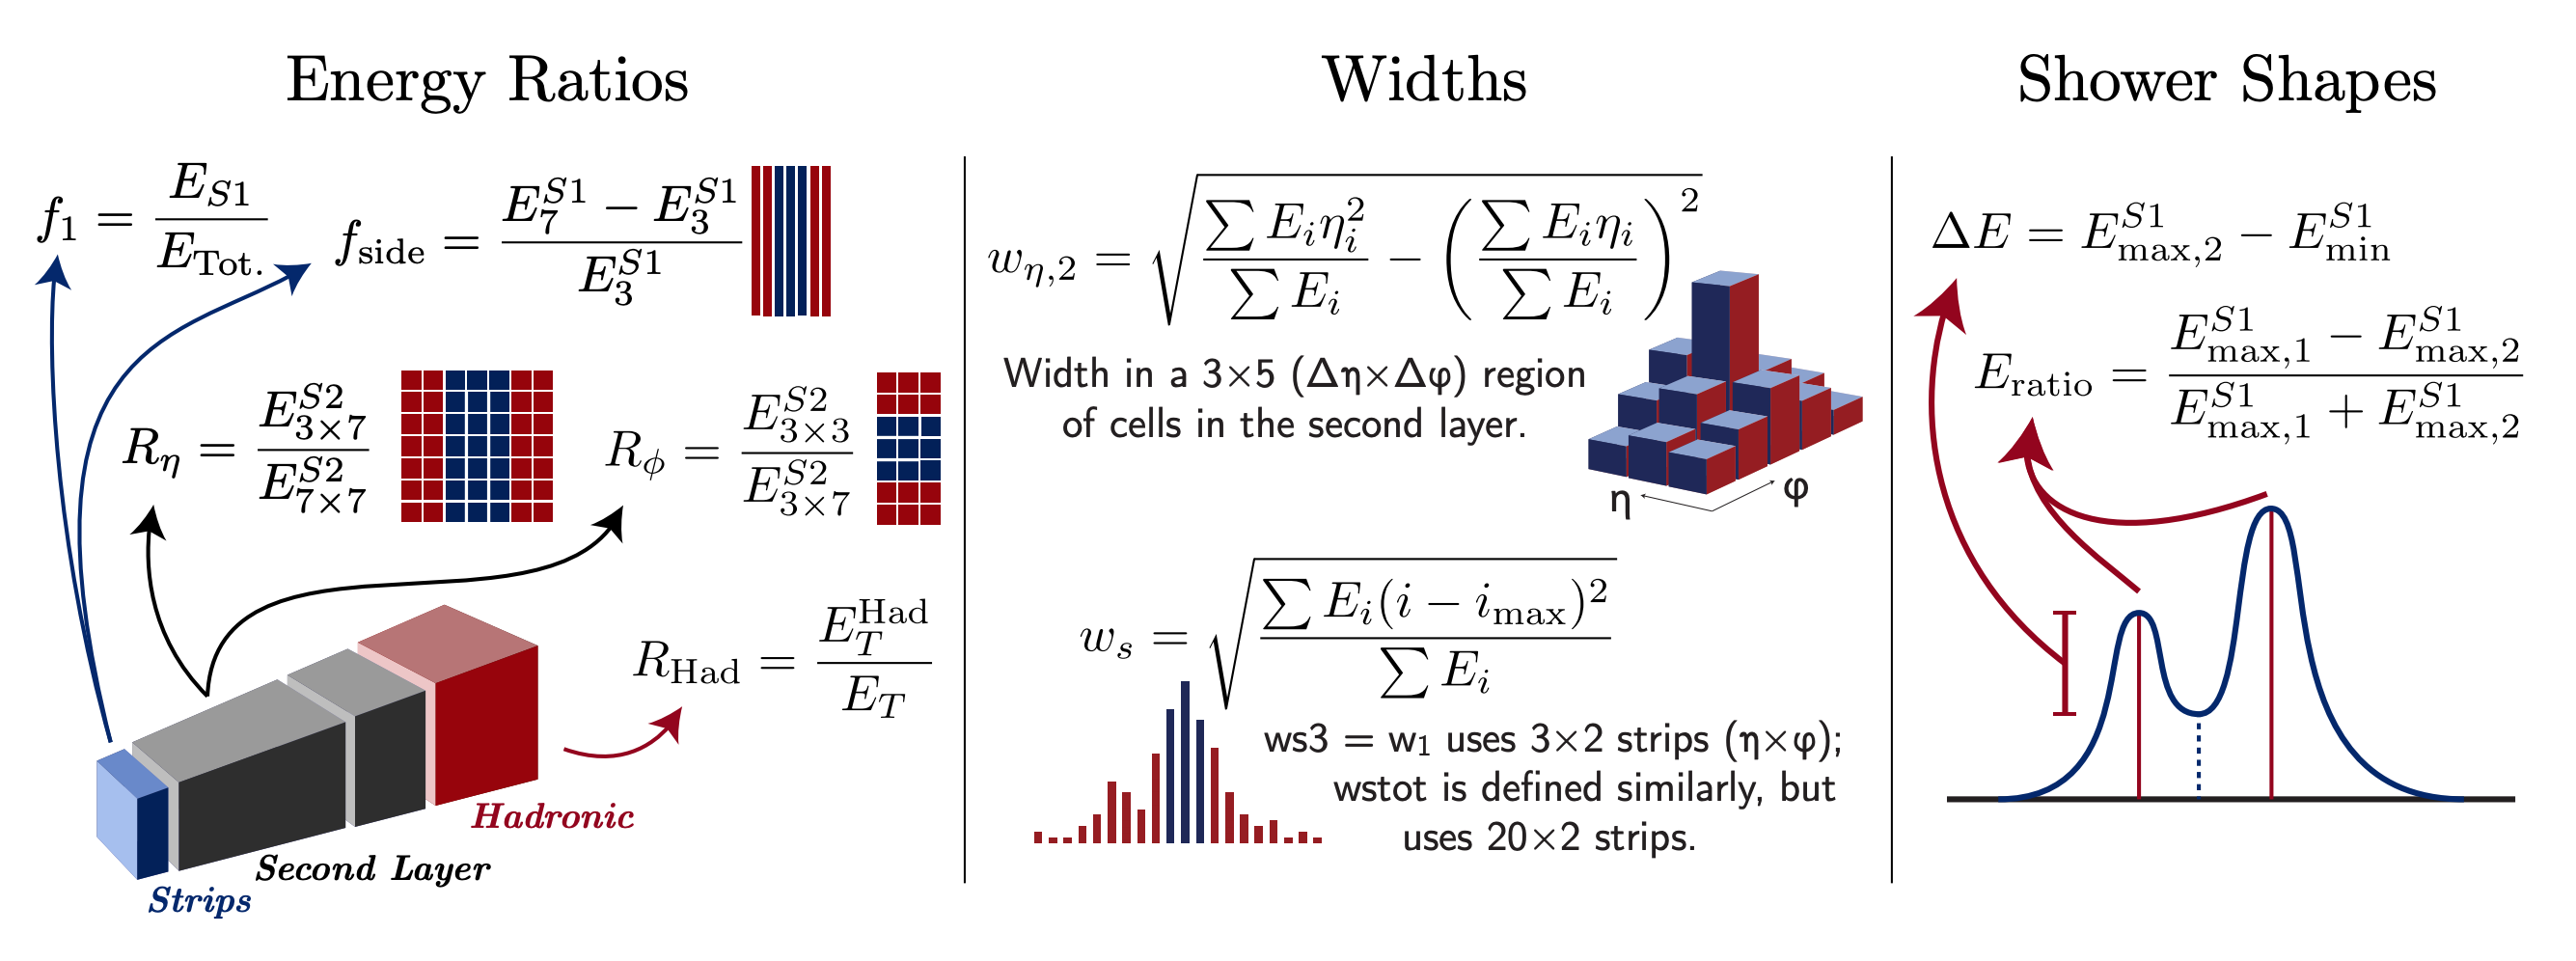
\includegraphics[width=.98\textwidth]{chapters/chapter4_photonID/images/ss-vars.png}
    \caption[Schematic of the shower shape variables used in the present cut-based photon identification.]
    {Schematic of the shower shape variables used in the present cut-based photon identification~\cite{ss-var-schematic}.}
    \label{fig:ss-vars-schematic}
\end{figure}

\begin{table}
    \centering
    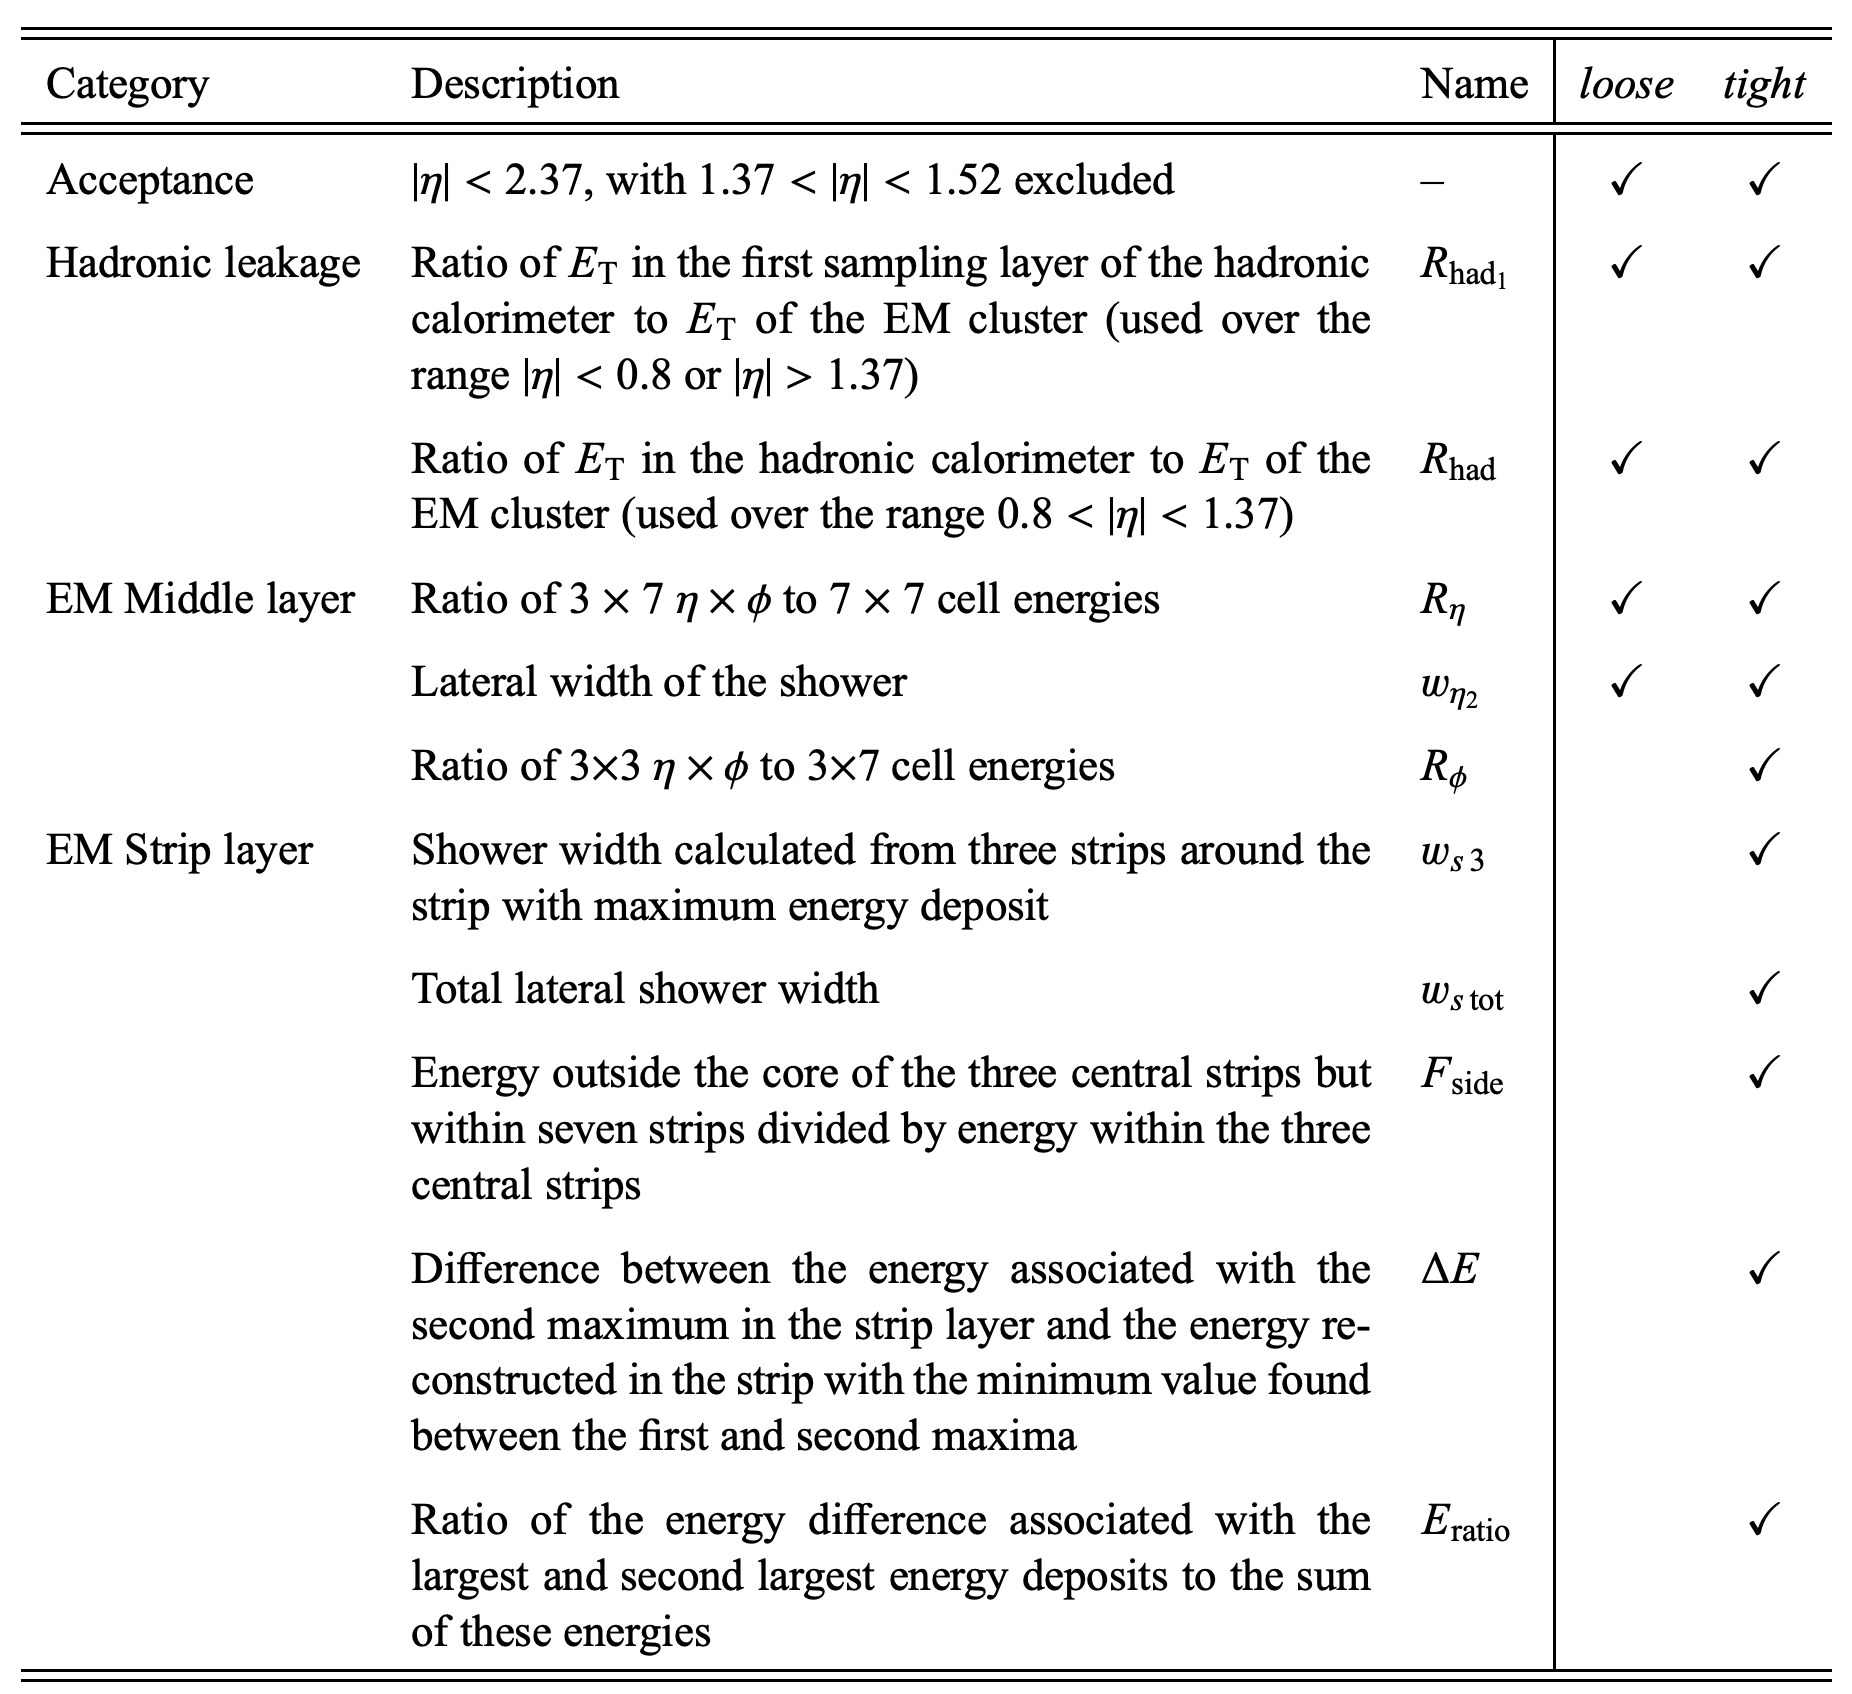
\includegraphics[width=.90\textwidth]{chapters/chapter4_photonID/images/ss-table.png}
    \caption[List of discriminating variables used in the present photon identification.]
    {List of discriminating variables used in the present photon identification~\cite{r1-photonID}.}
    \label{tab:ss-vars-table}
\end{table}

Cuts on these variables are derived in bins of \abseta. The intervals are 0.0, 0.6, 0.8, 1.15, 1.37, 1.52, 1.81, 2.01, 2.37, with a bin defined between each step (e.g. $[0.0,0.6)$, $[0.6,0.8)$, etc.) to account for the geometry of the calorimeter and the effects upstream material has on the shower shapes. The region $[1.37,1.52)$ is omitted, due to the transition crack between where the \gls{EMB} and \gls{EMEC} lies. In this region, there is considerable material before the \gls{EM} calorimeter, and is not considered for precision photon identification. The most recent iteration of the tight photon identification introduced binning in \pt, where bins are defined at 25, 30, 40, 50, 60, 80, 100, 125, 150, 175, 250, 500, and 1000 GeV. This provides increased signal efficiency at low \pt, and improved background rejection at high \pt.

This chapter describes an optimization to photon identification through two approaches. First, through adding additional discriminating variables to be used as inputs. This is done through investigating the use of observables of topological clusters, described in Section~\ref{sec:topo-clusters-yid}. Second, alternative methods of classification are studied, replacing the current univariate cut-based approach with a multivariate algorithm. This is shown in Section~\ref{sec:mva-yid}, in which a \gls{BDT} and a \gls{NN} are studied.


\section{MC Samples}\label{sec:photon-id-samples}

In optimization of photon identification, the aim is to discriminate prompt photons from various background sources. The predominant background is from decays inside of hadronic jets which result in non-prompt photons, such as $\pi^{0}\rightarrow \gamma \gamma$.

For these studies, a sample of leading-order $\gamma+$jet events from $qg \rightarrow q \gamma$ and $q\bar{q} \rightarrow g \gamma$ hard scattering, as well as events with prompt photons from quark fragmentation in \gls{QCD} dijet events is used. For background non-prompt photons in jets, a jet-jet sample with all tree-level $2\rightarrow2$ QCD processes is used, with $\gamma+$jet events containing prompt photons removed. Both samples are generated using \peight with the \texttt{A14} tune and \texttt{NNPDF2.3LO} PDF set. The simulation matched the detector conditions in the 2015 and 2016 data taking period. In both cases, an inclusive \texttt{OR} of loose single photon triggers is applied, with thresholds running as low as 10 GeV\footnote{The triggers applied are \texttt{HLT\_g*\_loose}}.

\subsection{Event Selection}

Selected events are required to have a photon with $\abseta < 2.37$, excluding the crack region ($1.37<\abseta<1.52$), and $\pt > \unit{25}{\GeV}$. In each event, the photon with the highest \pt is considered. For the signal single photon sample, \gls{MC} truth information is used to require the selected photon to be a prompt photon (\textit{truth-matched}), for the jet-jet background a prompt photon veto is applied to the selected photon (\textit{truth-vetoed}). 


\section{Topological Clusters}\label{sec:topo-clusters-yid}

Photon reconstruction is performed through a method known as ``topological clustering,'' which is described in Section~\ref{ssec:em-signatures}. In the calorimeter, energy depositions are clustered via this method, then these topo-clusters are merged into superclusters, which are ultimately the detector signature which may be defined as the photon. The reconstructed observables of these topological clusters, or \textit{moments}, can be used to characterize them. This section will discuss the use of these topological cluster moments in photon identification to better reject background from non-prompt photons.

In general, moments are given at order $n$ for a calorimeter cell variable, $v_{\text{cell}}$ as
\begin{equation}\label{eqn:moment-calculation}
    \langle v_{\text{cell}}^{n} \rangle = \frac{
        \sum_{\{i|E_{\text{cell},i}^{\text{EM}}>0\}}w^{\text{geo}}_{\text{cell},i} E_{\text{cell},i}^{\text{EM}} v_{\text{cell},i}^{n}
    }
    {
        \sum_{\{i|E_{\text{cell},i}^{\text{EM}}>0\}}w^{\text{geo}}_{\text{cell},i} E_{\text{cell},i}^{\text{EM}}
    }.
\end{equation}
The moments use \gls{EM} scale cell signals, $E_{\text{cell},i}^{\text{EM}}$, and the summation is performed over $i$ cells in a cluster. To restrict moment calculation to in-time signals, $E_{\text{cell},i}^{\text{EM}}$ must be greater than 0. The geometric signal weights are given by $w^{\text{geo}}_{\text{cell},i}$, which are introduced by cluster splitting. If proto-clusters have multiple local signal maxima with $E_{\text{cell}}^{\text{EM}} > \unit{500}{\MeV}$ in the \gls{EM} sampling layers, the cluster is split. Cells which are neighbors to multiple maxima are assigned in a weighted proportion to the two highest energy clusters, $E_{\text{clus},1}^{\text{EM}}$ and $E_{\text{clus},2}^{\text{EM}}$, after splitting the original topo-cluster. For cells of distances $d_1$ and $d_2$ to the center of the maxima, these are given by: 
\begin{equation}
    w^{\text{geo}}_{\text{cell,1}} = \frac{E_{\text{clus},1}^{\text{EM}}}{E_{\text{clus},1}^{\text{EM}} + r E_{\text{clus},2}^{\text{EM}}}
\end{equation}
\begin{equation}
    w^{\text{geo}}_{\text{cell,2}} = 1-w^{\text{geo}}_{\text{cell,1}}
\end{equation}
\begin{equation}
    r = \exp(d_1 -d_2).
\end{equation}
For cells not split between maxima, this value is 1. The used moments are all of order $n=1$ (centroids) or $n=2$ (spreads)~\cite{topo-cluster}.

\noindent\textbf{Number of Topo-Clusters}\\
\indent As described in Section~\ref{ssec:em-signatures}, superclusters are made up of one or more topo-clusters. Multiple topo-clusters in a supercluster can be a result of cluster splitting or bremsstrahlung radiation. In over 90\% of photon events, there is only 1 topo-cluster associated to the photon supercluster, shown in Figure~\ref{fig:num-clusters}. As a result, the quantities studied as inputs are all of the topo-cluster with the largest total energy (summed over constituent cells). Additionally, the number of topo-clusters is on average fewer for prompt photons than fakes, so this value is used as an input into the classification.


\begin{figure}[htb]
    \centering
    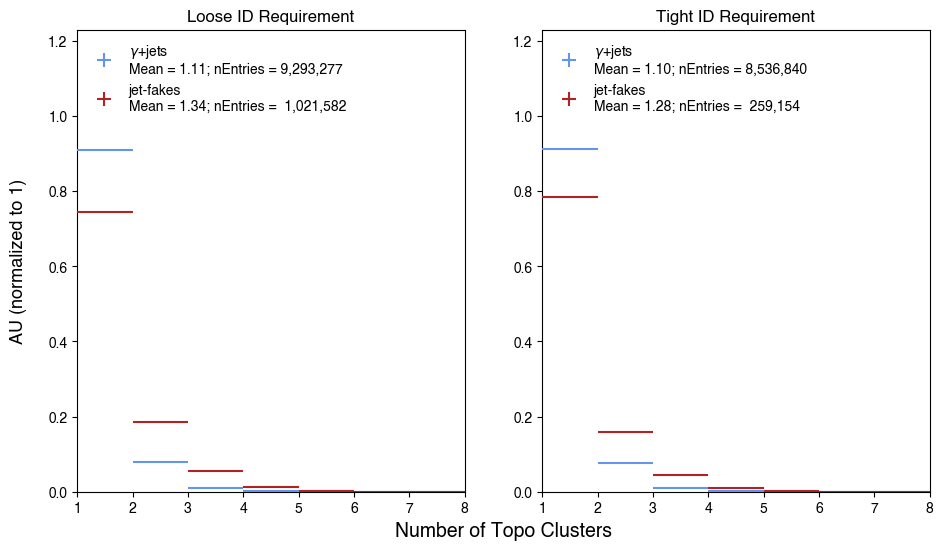
\includegraphics[width=\textwidth]{chapters/chapter4_photonID/images/hists/y_nTopoClusters.png}
    \caption[Number of topo-clusters in unconverted photon superclusters]
    {Number of topo-clusters in unconverted photon superclusters in truth-matched $\gamma+$jet events and truth-vetoed jet fake events. Both prompt and fake photons predominantly just have 1 topo-cluster per supercluster. This is more true for prompt photons, which on fewer topo-clusters on average than fakes.} 
    \label{fig:num-clusters}
\end{figure}


\noindent\textbf{Shape Information}\\
\indent The size of the topo-cluster indexed $i$ is parameterized by moments in $r_i$ and $\lambda_i$, which are defined as:

\begin{equation}
    r_i = |(\vec{x_i} - \vec{c}) \times \vec{s}| \text{\hspace{2em}(radial distance to shower axis)} \\
\end{equation}
\begin{equation}
    \lambda_i = (\vec{x_i} - \vec{c}) \cdot \vec{s} \text{\hspace{2em}(longitudinal distance to shower center of gravity)},
\end{equation}
where $\vec{s}$ is the shower axis and $\vec{c}$ is the center of gravity. The center of gravity, $\vec{c}$, is calculated using Equation~\ref{eqn:moment-calculation}, using the first moments of the Cartesian coordinates specifying calorimeter cell centers. The locations are in the frame of reference of the detector with the \gls{IP} at $(x,y,z)= (0,0,0)$. The shower axis measures the direction of flight of the particle and is given by:
\begin{equation}
    \mathcal{C}_{uv} = \frac{1}{\mathcal{W}} \sum\limits_{\{i|E_{\text{cell},i}^{\text{EM}} >0\}}(w^{\text{geo}}_{\text{cell,i}}, E_{\text{cell},i}^{\text{EM}})^2 (u_i - \langle u \rangle)(v_i - \langle v \rangle)
\end{equation}
for every permutation of $u,v \in \{x,y,z\}$ and 
\begin{equation}
    \mathcal{W} = \sum\limits_{\{i|E_{\text{cell},i}^{\text{EM}} >0\}} (w^{\text{geo}}_{\text{cell,i}}, E_{\text{cell},i}^{\text{EM}})^2.
\end{equation}
Then, the values of $\mathcal{C}_{uv}$ can be used to create a $3 \times 3$ matrix, $\mathbf{C}=[\mathcal{C}_{uv}]$. The shower axis, $\vec{s}$, is the eigenvector of $\boldsymbol{C}$ closest to the direction $\vec{c}$ from the \gls{IP} to the center of gravity of the topo-cluster. If the angular distance between $\vec{c}$ and $\vec{s}$ is larger than 20 degrees, then $\vec{c}$ is used as the shower axis.

 Through this parameterization, the topo-cluster can be analyzed as a spheroid, with the second moments in $r$ and $\lambda$ as the extensions; $\sqrt{\langle \lambda^2 \rangle}$ is the semi-major axis in depth (along the shower axis), $\sqrt{\langle r^2 \rangle}$ is the semi-major axis in width. The distribution of these two parameters are shown for the leading topo-cluster in Figures~\ref{fig:topo-secondLambda} and~\ref{fig:topo-secondR}, after applying the current loose and tight photon identification criteria. Differences remaining in these distributions after applying the current identification is information the current criteria does not capture, and can bring additional discriminating power.

 \begin{figure}[!htbp]
    \centering
    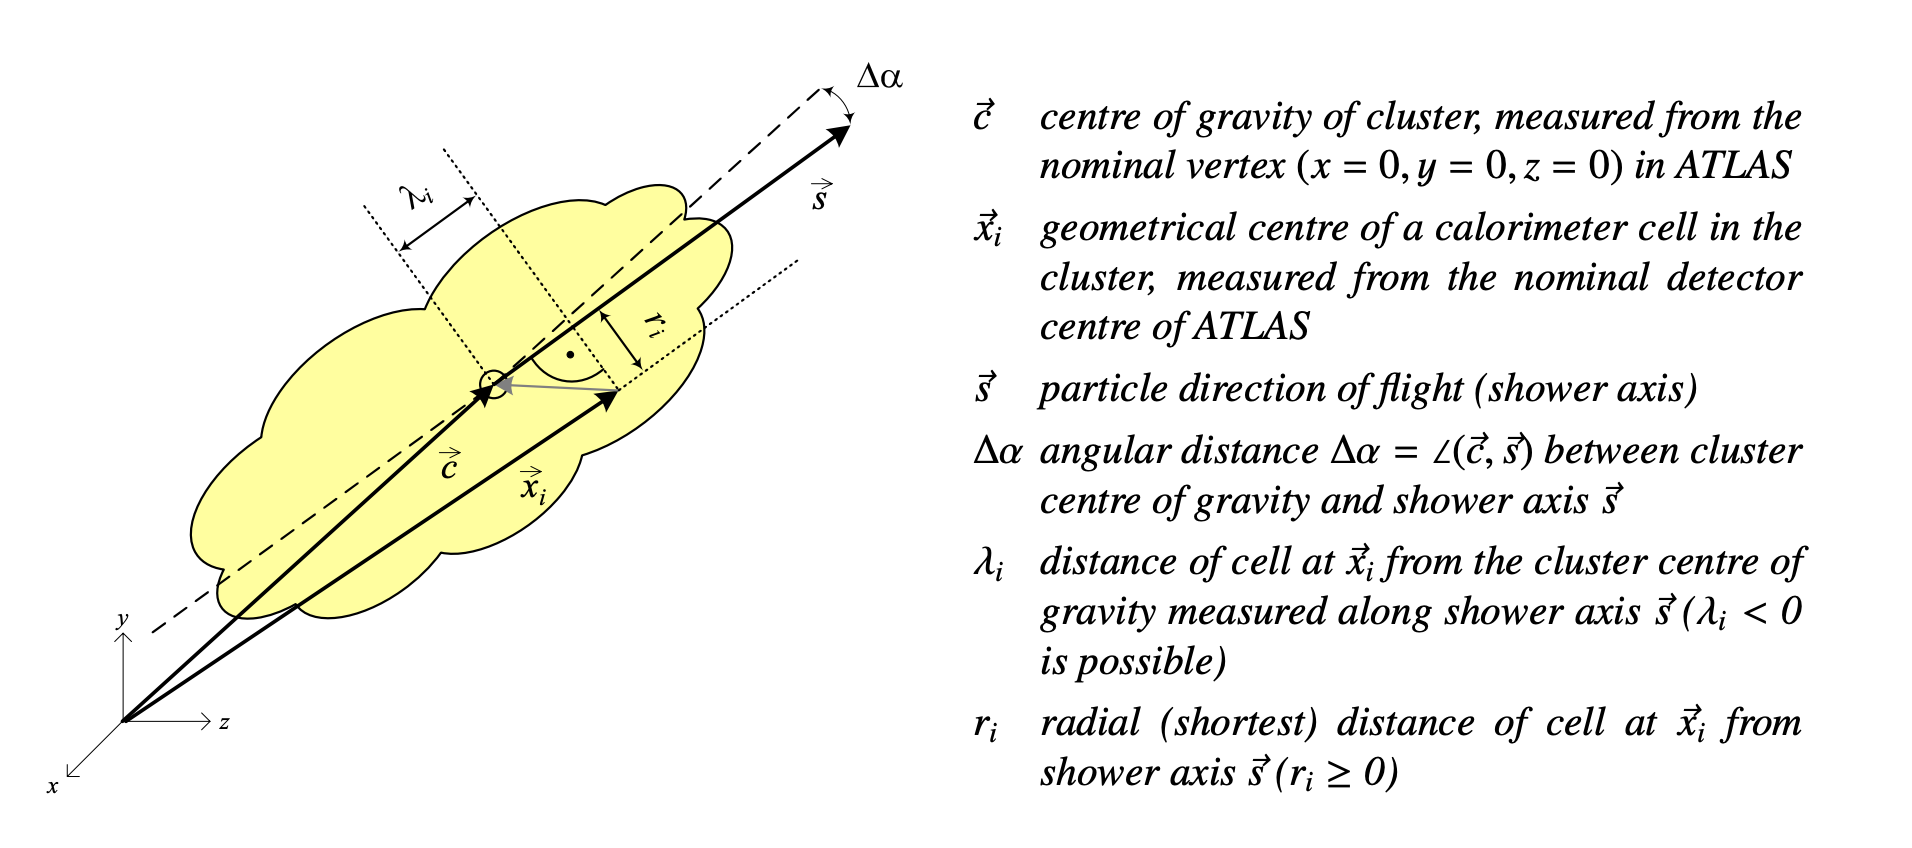
\includegraphics[width=.90\textwidth]{chapters/chapter4_photonID/images/geom-moments.png}

    \caption[The geometric moments and relevant parameters for topo-clusters.]
    {The geometric moments and relevant parameters for topo-clusters~\cite{topo-clustering-r1}.}
    \label{fig:topo-geom}
\end{figure}

 \begin{figure}[!htbp]
    \centering
    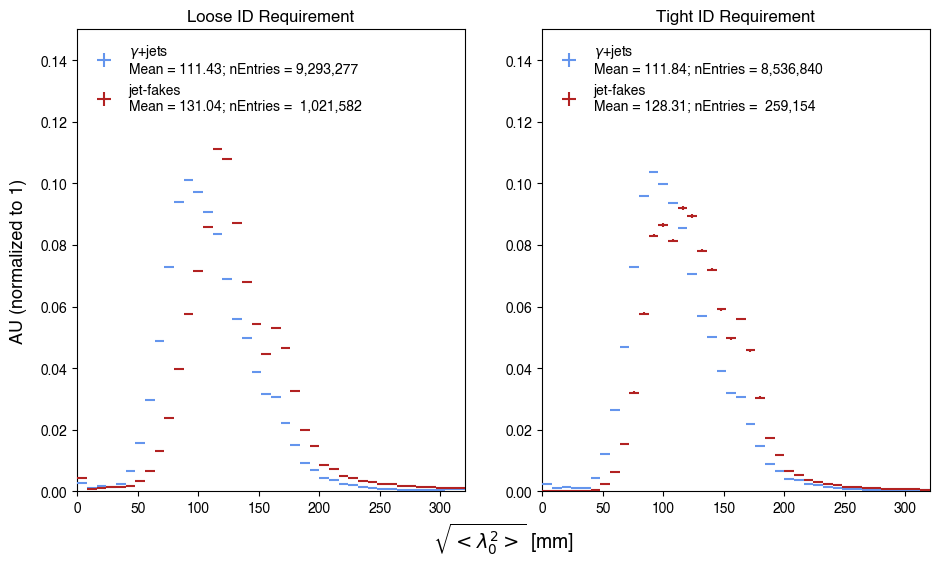
\includegraphics[width=\textwidth]{chapters/chapter4_photonID/images/hists/y_topoCluster0_secondLambda.png}
    \caption[The distribution of the semi-major axis in depth, $\sqrt{\langle \lambda^2 \rangle}$, for the leading topo-cluster]{The distribution of the semi-major axis in depth, $\sqrt{\langle \lambda^2 \rangle}$, for the leading topo-cluster in truth-matched $\gamma+$jet events and truth-vetoed jet fake events.}
    \label{fig:topo-secondLambda}

\end{figure}

\begin{figure}[!htbp]
    \centering 
    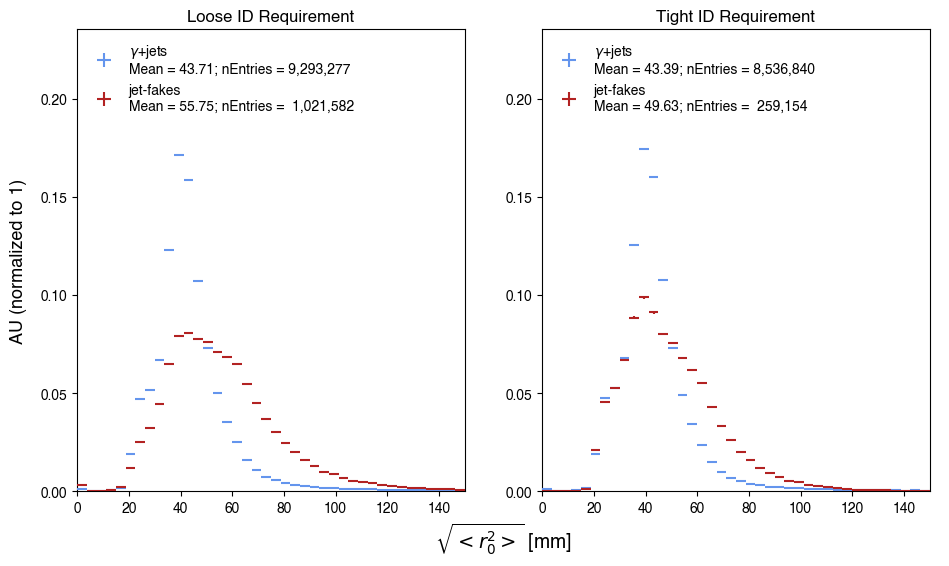
\includegraphics[width=\textwidth]{chapters/chapter4_photonID/images/hists/y_topoCluster0_secondR.png}
    \caption[The distribution of the semi-major axis in width, $\sqrt{\langle r^2 \rangle}$, for the leading topo-cluster]{The distribution of the semi-major axis in width, $\sqrt{\langle r^2 \rangle}$, for the leading topo-cluster in truth-matched $\gamma+$jet events and truth-vetoed jet fake events.}
    \label{fig:topo-secondR}
\end{figure}


%\footnote{Plots in this chapter are created using the \texttt{Matplotlib} python library~\cite{matplotlib}}


\noindent\textbf{Location Information}\\
\indent The location of the topo-cluster is calculated from the first moments of the three Cartesian coordinates, describing the position of $\vec{c}$. Due to azimuthal symmetry in the detector, the key locational component of topo-clusters is the depth in the calorimeter. Thus, this location can be described via $\lambda_{clus}$, the distance of the center of gravity from the front face of the calorimeter. This distribution is shown in Figure~\ref{fig:topo-centerLambda}.

\begin{figure}[!htbp]
    \centering 
    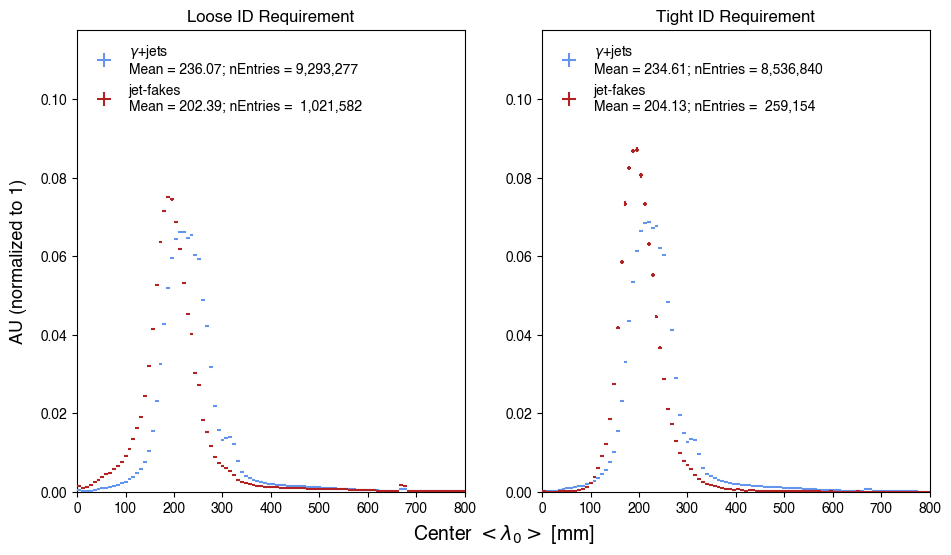
\includegraphics[width=\textwidth]{chapters/chapter4_photonID/images/hists/y_topoCluster0_centerLambda.png}
    \caption[The distribution of the centroid depth ($<\lambda_{0}>$) of the leading topo-cluster]{The distribution of the centroid depth ($<\lambda_{0}>$) of the leading topo-cluster in truth-matched $\gamma+$jet events and truth-vetoed jet fake events.}
    \label{fig:topo-centerLambda}
\end{figure}

A visualization of the geometric moments, both location and shape can be found in Figure~\ref{fig:topo-geom}, with relevant spacial parameters (e.g. $\vec{c}$, $\vec{s}$, etc.) shown and defined.



\noindent\textbf{Additional Moments}\\
\indent Beyond the shape and location information, there are several other moments that can be used. Two are considered as inputs, cluster isolation and \gls{EM} probability.

The signal thresholds built into the topological clustering algorithm are constructed to suppress noise, but lead to signal losses at the perimeter of clusters. The isolation moment, $f_{\text{iso}}$, measures the degree of isolation of a cluster. It is constructed as a weighted fraction of the sampling layer energy ($E_{s}^{\text{EM}}$) of non-clustered neighbor cells on the perimeter of the topo-cluster in the sampling layer. It is given by

\begin{equation}
    f_{\text{iso}} = \frac
    {
    \sum_{S \in \{ \text{samplings with} E_{s}^{\text{EM}} > 0 \} }  
    E_{s}^{\text{EM}} N_{\text{cell},s}^{\text{noclus}} / N_{\text{cell},s}^{\text{neighbor}}
    } 
    {
        \sum_{S \in \{ \text{samplings with} E_{s}^{\text{EM}} > 0 \} }
    }.
\end{equation}

Here, $N_{\text{cell},s}^{\text{noclus}} / N_{\text{cell},s}^{\text{neighbor}}$ is the ratio of unclustered perimeter cells to the total number of perimeter cells for a given cluster. This is summed across all sampling layers with positive energy, $s$. For the signal and background samples, the isolation is shown using the existing loose and tight identification criteria in Figure~\ref{fig:topo-isolation}.

\begin{figure}[htb]
    \centering 
    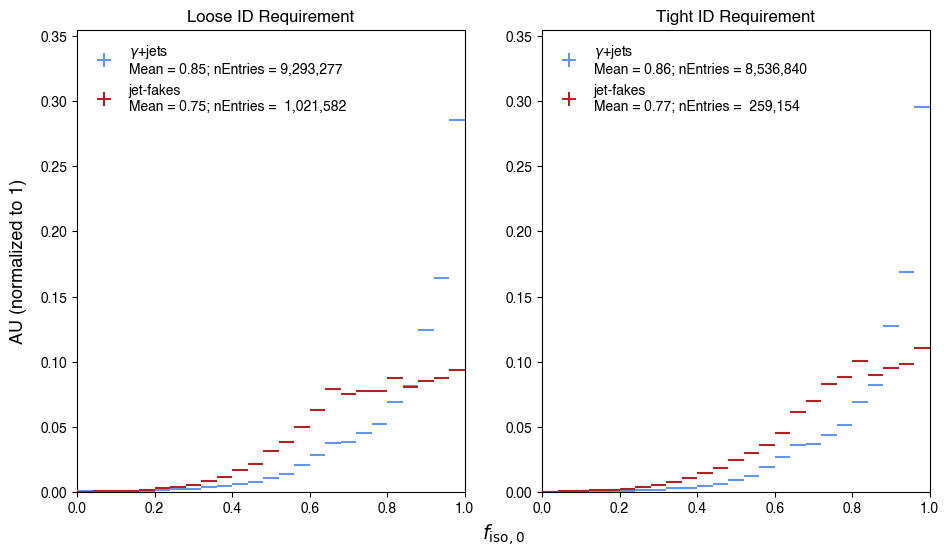
\includegraphics[width=\textwidth]{chapters/chapter4_photonID/images/hists/y_topoCluster0_isolation.png}
    \caption[The distribution of the isolation moment of the leading topo-cluster]{The distribution of the isolation moment of the leading topo-cluster in truth-matched $\gamma+$jet events and truth-vetoed jet fake events}
    \label{fig:topo-isolation}
\end{figure}

Energy losses in topo-clusters are corrected through a method known as \gls{LCW}~\cite{lcw-calib}. Since energy losses differ between hadronic and electromagnetic deposits, \gls{LCW} includes a step where the likelihood that a topo-cluster originates from an electromagnetic shower is evaluated. The likelihood is defined through measuring the efficiency for detecting an EM-like cluster in bins of four other topo-cluster observables, defined by

\begin{equation}
    \mathfrak{O}_{\text{clus}}^{\text{class}} = \{
        E_{\text{clus}}^{\text{EM}},
        \eta_{\text{clus}},
        \log_{10}(\rho_{\text{clus}} / \rho_{\text{0}}) - \log_{10}(E_{\text{clus}}^{\text{EM}} / E_{\text{0}}),
        \log_{10}(\lambda_{\text{clus}} / \lambda_{\text{0}})
    \}
\end{equation}
where $\rho_0 = 1$ MeV mm$^{-3}$, $E_0 = \unit{1}{\MeV}$, $\lambda_{0} = \unit{1}{\mm}$. These bins (denoted $ijkl$) can then be used to define the likelihood, $ \mathcal{P}_{\text{clus}}^{\text{EM}}$, in each bin as
\begin{equation}
    \mathcal{P}_{\text{clus}}^{\text{EM}} ( E_{\text{clus}}^{\text{EM}}, \eta_{\text{clus}}, \rho_{\text{clus}} / E_{\text{clus}}^{\text{EM}}, \lambda_{\text{clus}}) \mapsto \mathcal{P}_{\text{clus}, ijkl}^{\text{EM}}  = \frac{\epsilon^{\pi^0}_{ijkl}}{ \epsilon^{\pi^0}_{ijkl} + 2\epsilon^{\pi^\pm}_{ijkl}},
\end{equation}
where $\epsilon^{\pi^0(\pi^\pm)}_{ijkl}$ is the efficiency, defined as
\begin{equation}
    \epsilon^{\pi^0(\pi^\pm)}_{ijkl} = \frac{ N^{\pi^0(\pi^\pm)}_{ijkl} }{N^{\pi^0(\pi^\pm)}_{ij}}
\end{equation}
for $N^{\pi^0(\pi^\pm)}_{ijkl}$ topo-clusters in a given bin $ijkl$ and $N^{\pi^0(\pi^\pm)}_{ij}$ topo-clusters in bin $ij$ of the $(E_{\text{clus}}^{\text{EM}}, \eta_{\text{clus}})$ phase space. This likelihood, $\mathcal{P}_{\text{clus}}^{\text{EM}}$, by definition is bounded from 0 to 1, and considered as an input. This distribution is shown in Figure~\ref{fig:topo-emProb}, with both the current loose and tight photon identification criteria applied.

\begin{figure}[htb]
    \centering 
    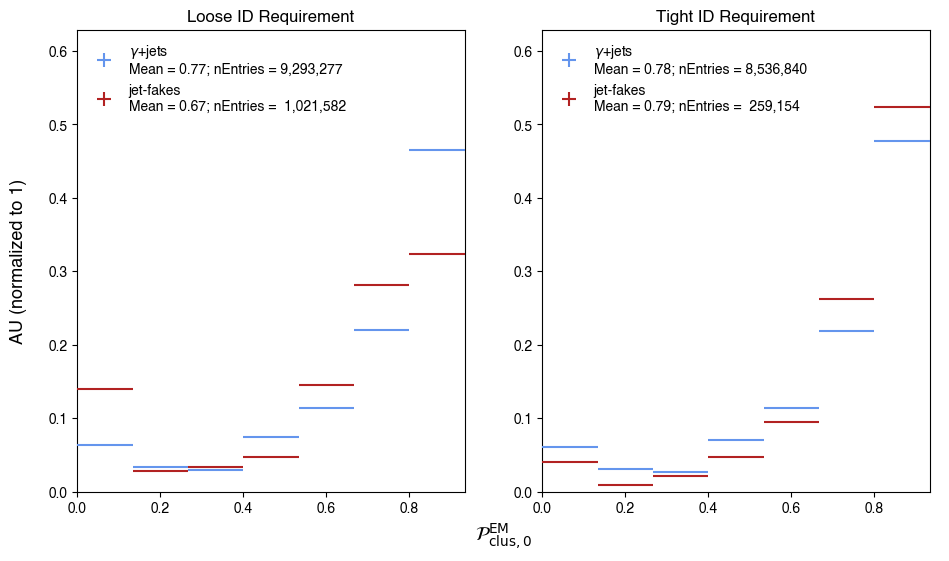
\includegraphics[width=\textwidth]{chapters/chapter4_photonID/images/hists/y_topoCluster0_emProbability.png}
    \caption[The distribution of the \gls{EM} probability moment of the leading topo-cluster]{The distribution of the \gls{EM} probability moment of the leading topo-cluster in truth-matched $\gamma+$jet events and truth-vetoed jet fake events}
    \label{fig:topo-emProb}
\end{figure}


\subsection{Data-MC Comparison}\label{ssec:yid-datamc}
In order to ensure that the topological clusters are properly modeled in the \gls{MC} simulation, the variables investigated are compared to data. To do so, the present tight photon ID is applied to both the \gls{MC} simulation and data. Data from the 2015+2016 data-taking period is considered, collected using a set of single-photon triggers with loose identification requirements matching those applied to the \gls{MC} samples, running as low as 10 GeV. As before, photons in \gls{MC} must correspond to a truth photon. Comparisons for $\sqrt{\lambda_{0}^2}$ and $\sqrt{r_{0}^2}$ are shown in Figure~\ref{fig:data-mc-secondLambda} and~\ref{fig:data-mc-secondR}, respectively. Comparisons for the remaining input variables considered are included into Appendix~\ref{app:datamc} for both converted and unconverted photons.

In general, the \gls{MC} models the unconverted photons well, with the exception of the isolation, particularly in the most central bin and beyond the crack. For converted photons, $\sqrt{r_{0}^2}$ modeling differs between data and \gls{MC}, and isolation differs considerably, particularly in the most central bin. On average converted photons have more topo-clusters per photon object, meaning they suffer more from cluster splitting, which influences these effects.


\begin{figure}[!thp]
    \centering
    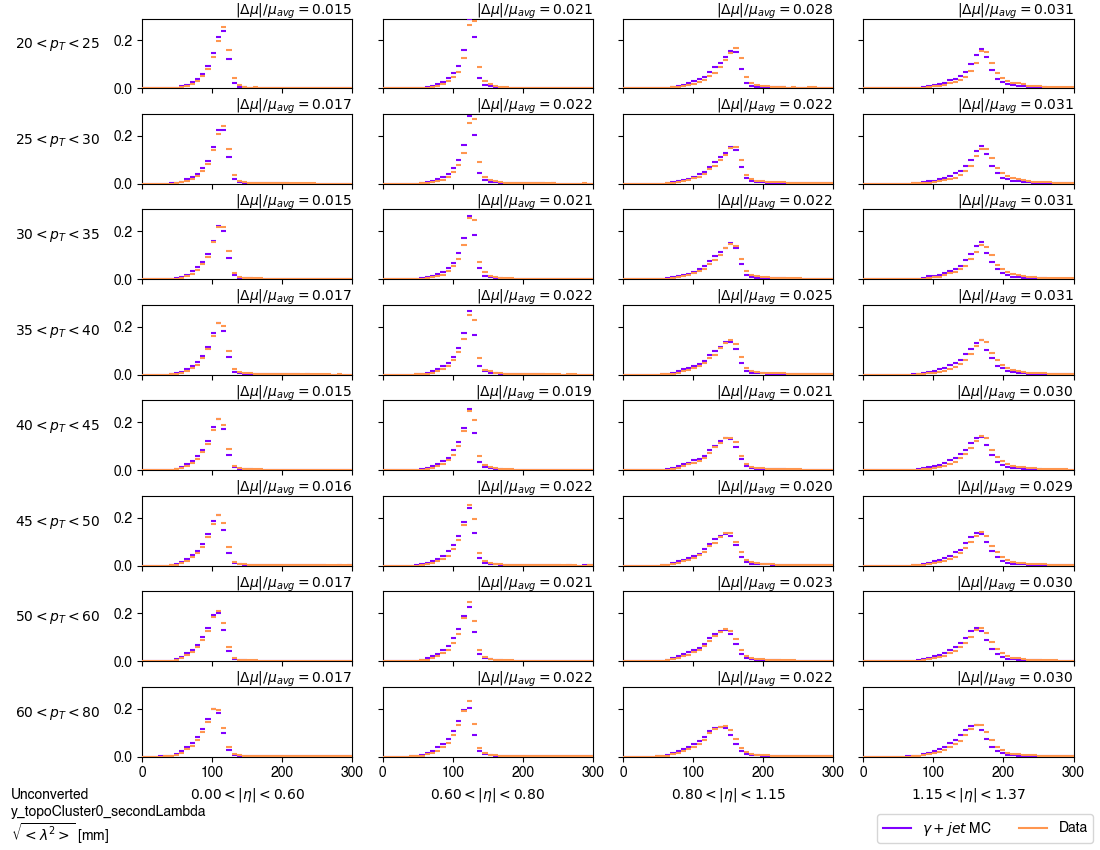
\includegraphics[width=.74\textwidth]{chapters/chapter4_photonID/images/y_topoCluster0_secondLambda_Unconverted_lowerEta.png}
    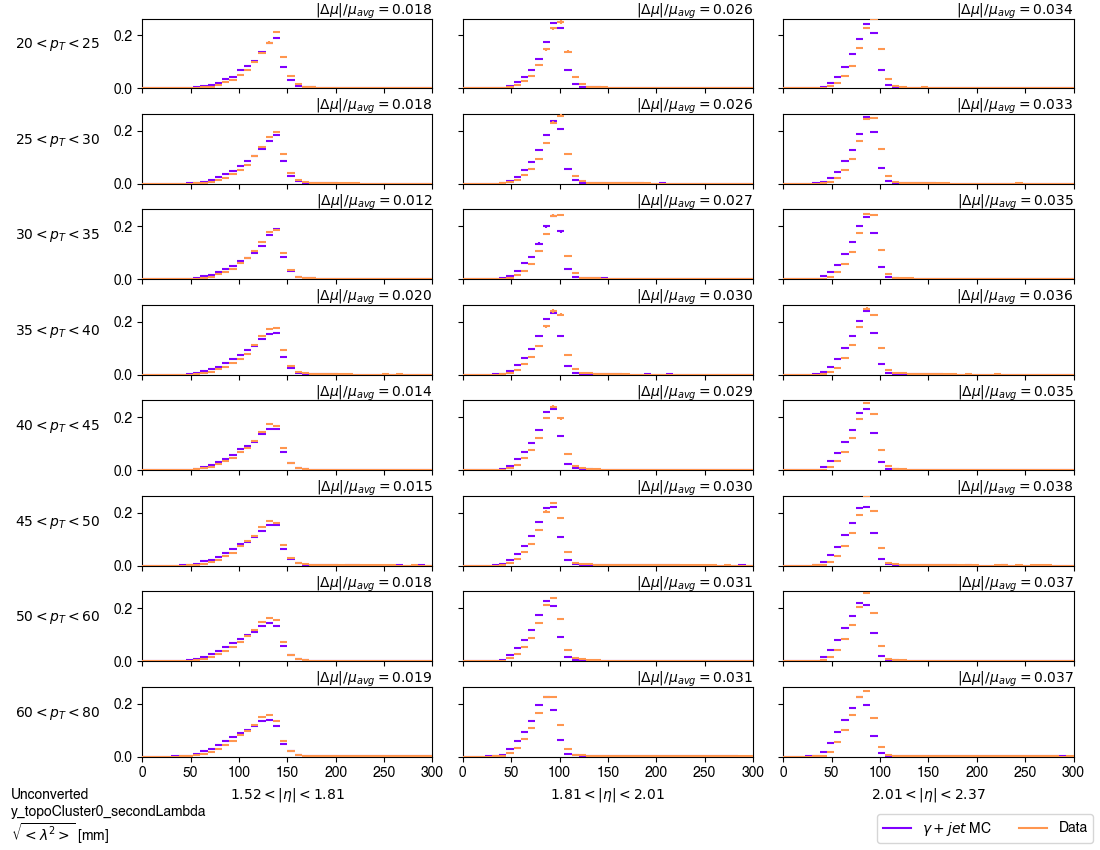
\includegraphics[width=.74\textwidth]{chapters/chapter4_photonID/images/y_topoCluster0_secondLambda_Unconverted_upperEta.png}
    \caption[Data-MC comparison of the semi-major axis in depth of the leading topo-cluster ($\sqrt{\lambda_0^2}$) for unconverted photons]{Data-MC comparison of the semi-major axis in depth of the leading topo-cluster ($\sqrt{\lambda_0^2}$) for unconverted photons. The current tight identification is applied to both samples, and the \gls{MC} requires truth-matched photons. The absolute difference of the distribution means normalized to their average mean, $|\Delta \mu|/\mu_{avg}$ is shown.}
    \label{fig:data-mc-secondLambda}
\end{figure}
\begin{figure}[!thp]
    \centering
    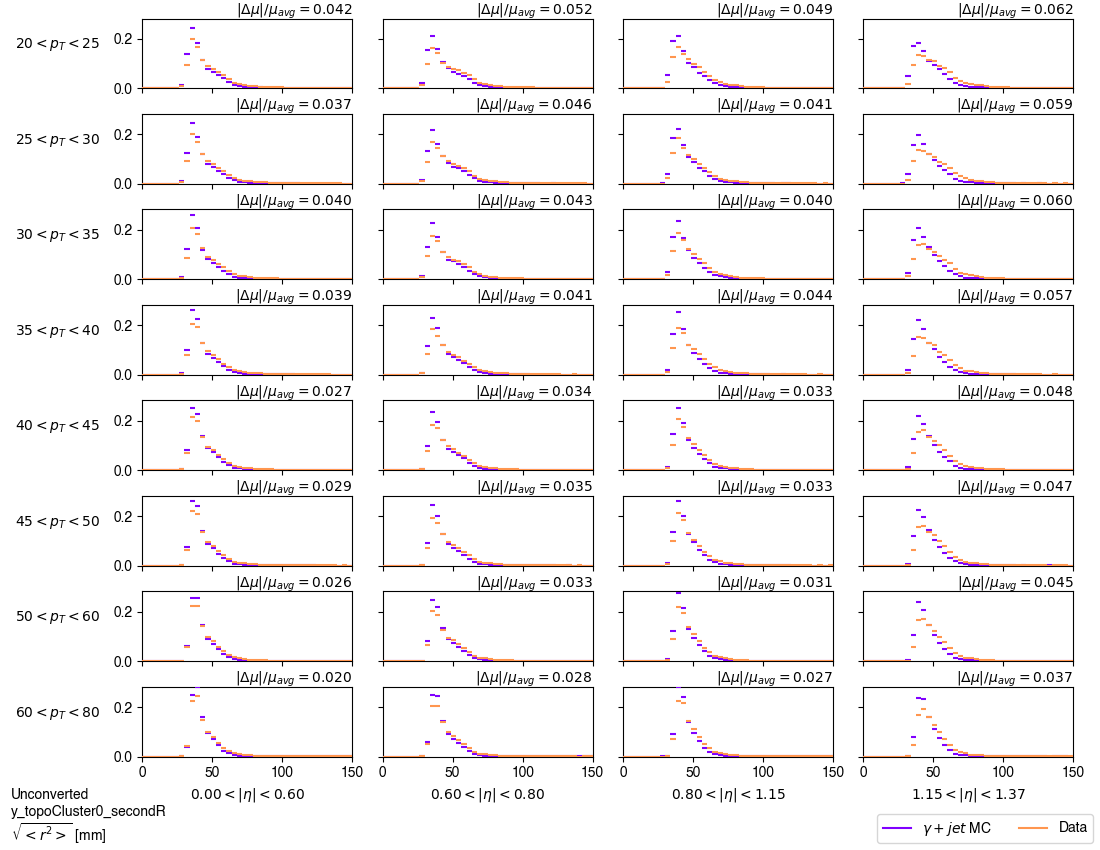
\includegraphics[width=.74\textwidth]{chapters/chapter4_photonID/images/y_topoCluster0_secondR_Unconverted_lowerEta.png}
    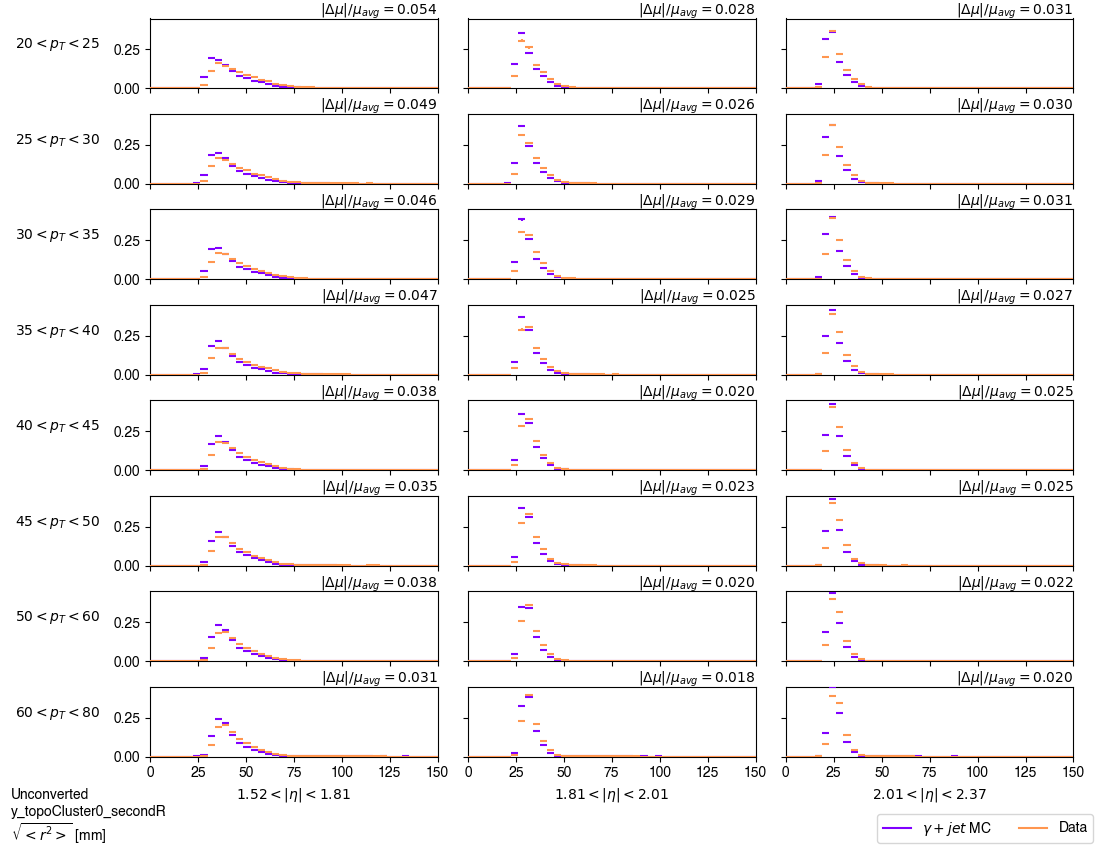
\includegraphics[width=.74\textwidth]{chapters/chapter4_photonID/images/y_topoCluster0_secondR_Unconverted_upperEta.png}
    \caption[Data-MC comparison of the semi-major axis in width of the leading topo-cluster ($\sqrt{r_0^2}$) for unconverted photons]{Data-MC comparison of the semi-major axis in width of the leading topo-cluster ($\sqrt{r_0^2}$) for unconverted photons.The current tight identification is applied to both samples, and the \gls{MC} requires truth-matched photons. The absolute difference of the distribution means normalized to their average mean, $|\Delta \mu|/\mu_{avg}$ is shown.}
    \label{fig:data-mc-secondR}
\end{figure}
% TODO: split these figs?

\noindent\textbf{Correlations}\\
\indent The correlations of the topo-cluster variables to each other, to the shower shape variables, and to the isolation working points are evaluated. The correlations between variables are checked since highly correlated do not bring new information, and thus are not useful for adding to photon identification methods. Photon identification and isolation must be uncorrelated in order to define the regions used for 2x2D sideband methods~\cite{2x2d-definition}, as correlations can affect the purity estimation. These correlations are shown for both the $\gamma$+jet in Figure~\ref{fig:photonid-corrs-sig} and for the jet-fakes sample in Figure~\ref{fig:photonid-corrs-bkg}. The added variables have low correlation to the isolation working points with the exception of the topo-cluster isolation, which is $\sim$40\% correlated to the working points. Additionally the topo-cluster variables have some correlation to one another, particularly the ones with shape information, but in general are comparable to the level of correlation between the shower shape variables.

\begin{figure}[!hp]
    \centering
    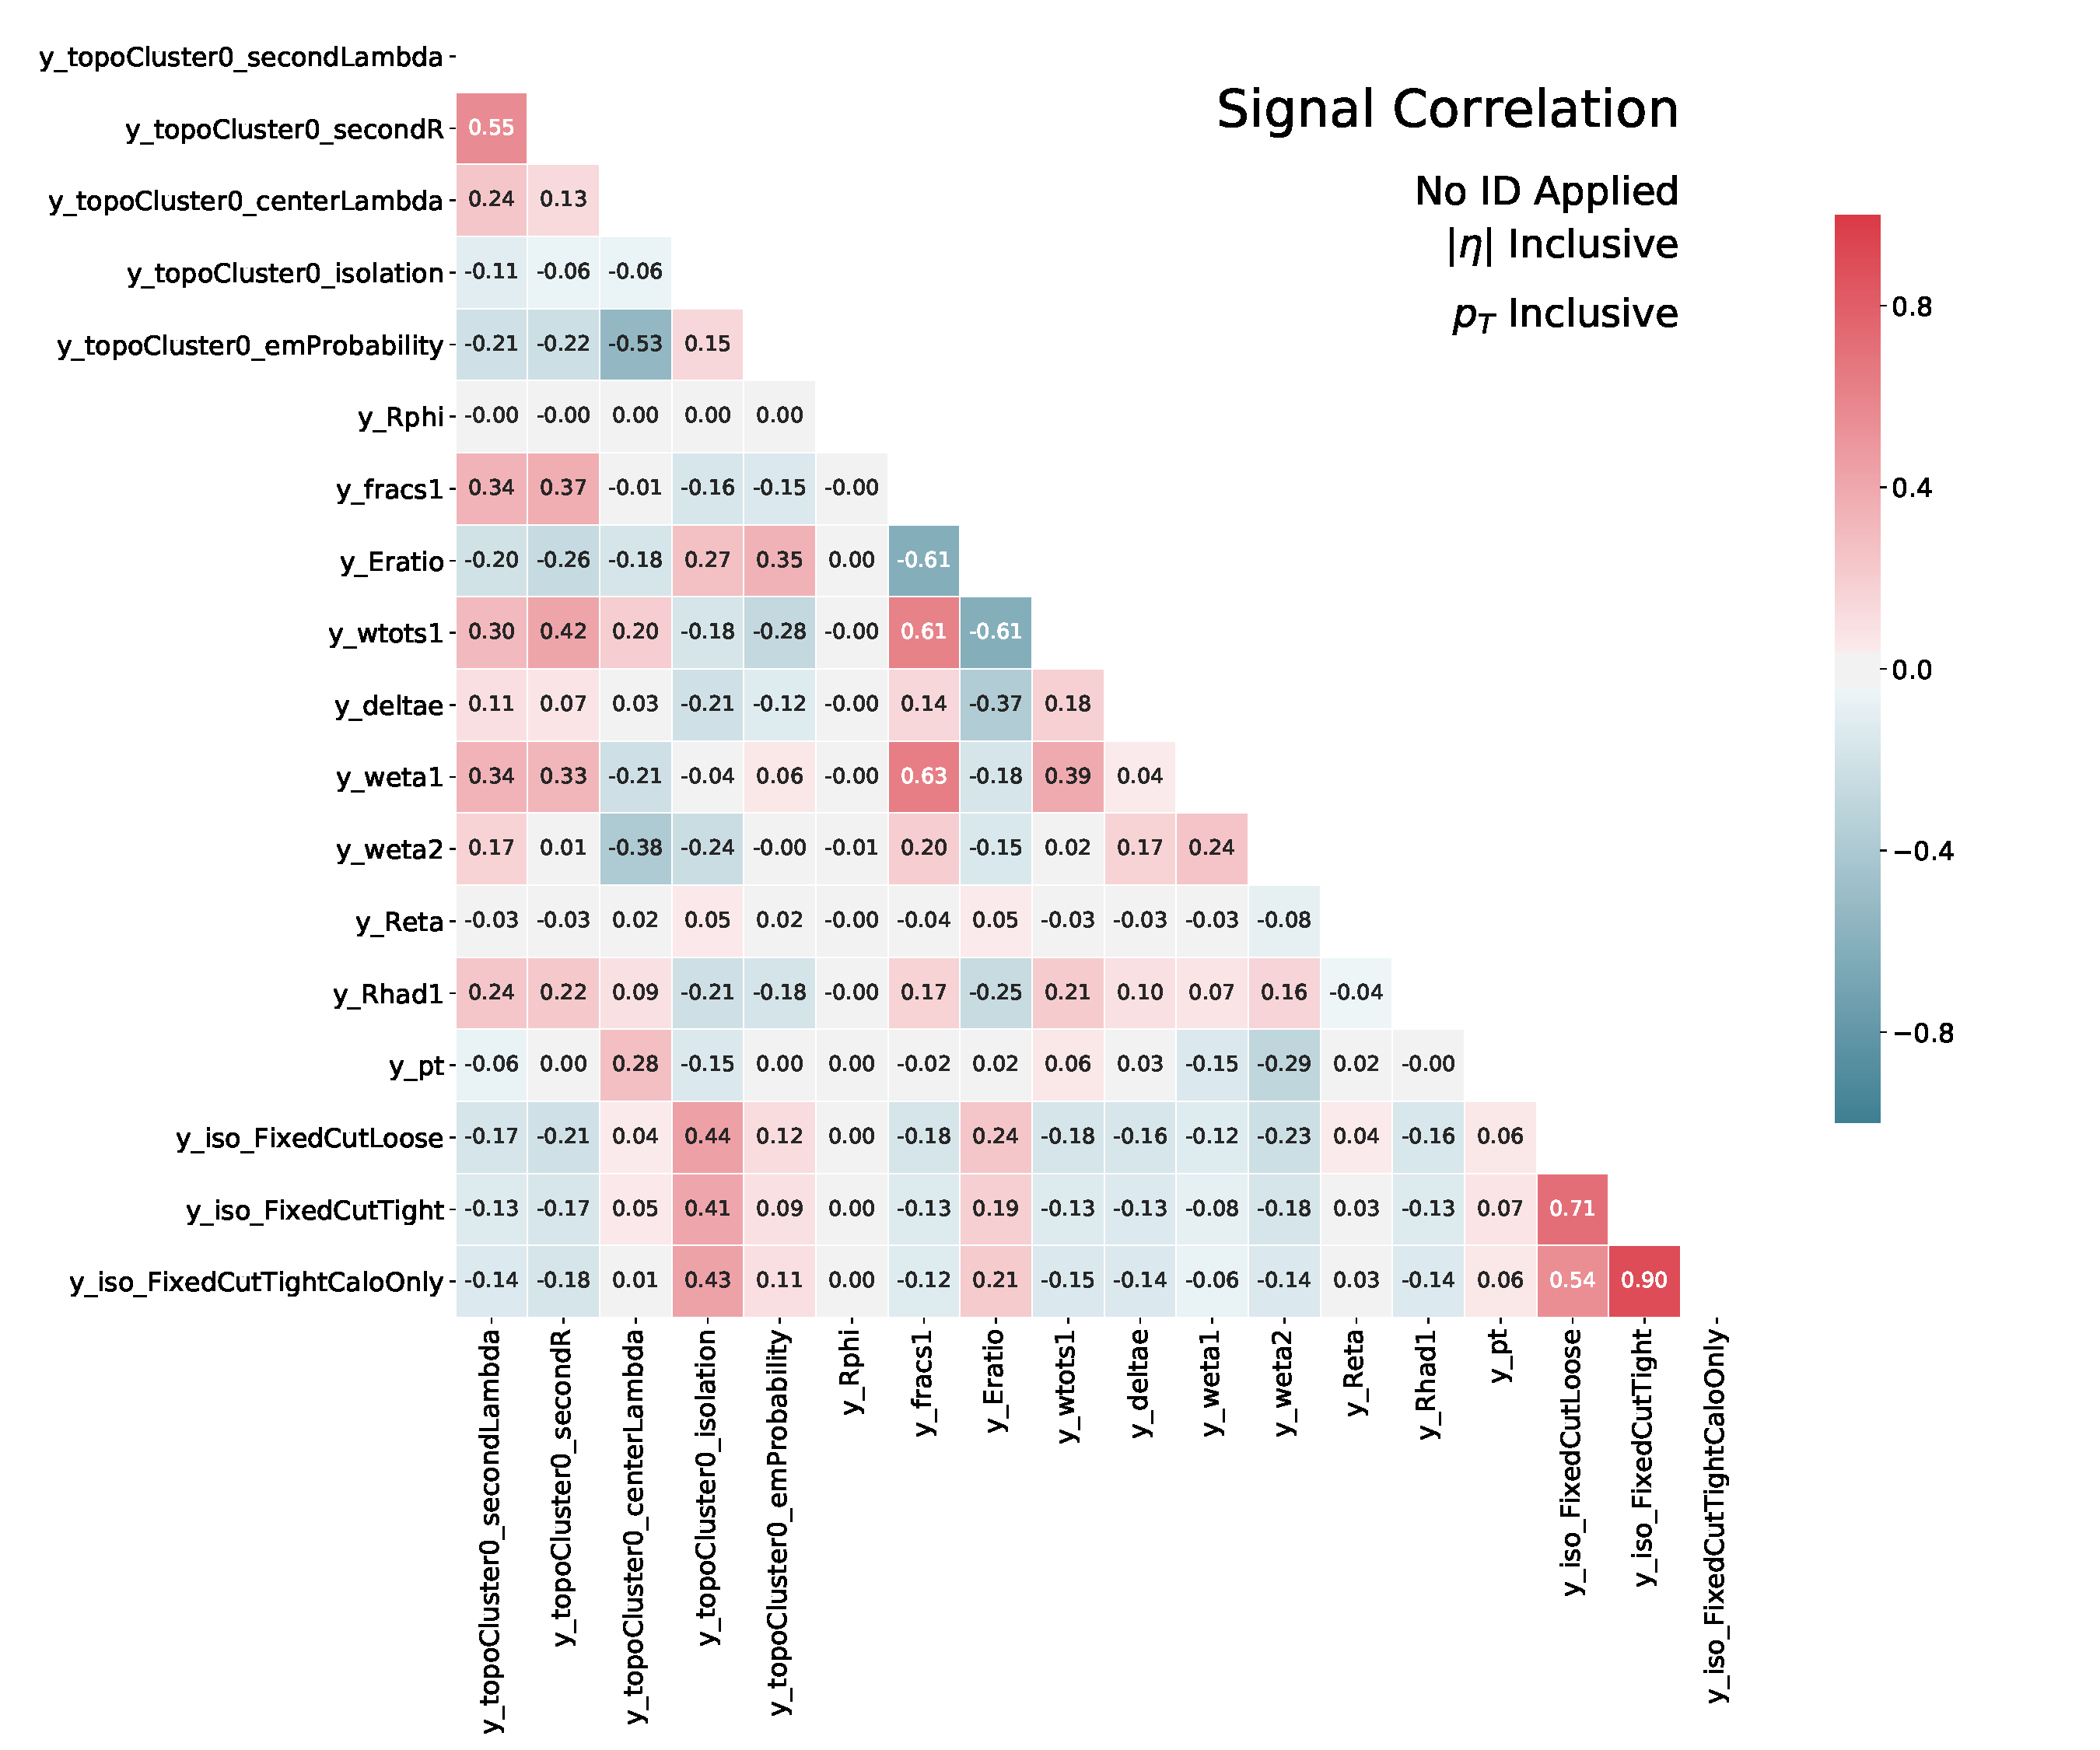
\includegraphics[width=\textwidth]{chapters/chapter4_photonID/images/sig_none_corr.pdf}
    \caption[Correlation values between the shower shape variables, topological cluster variables, and isolation working points for the $\gamma$+jet sample] {Correlation values between the shower shape variables, topological cluster variables, and isolation working points for the $\gamma$+jet sample.}
    \label{fig:photonid-corrs-sig}
\end{figure}

\begin{figure}[!hp]
    \centering
    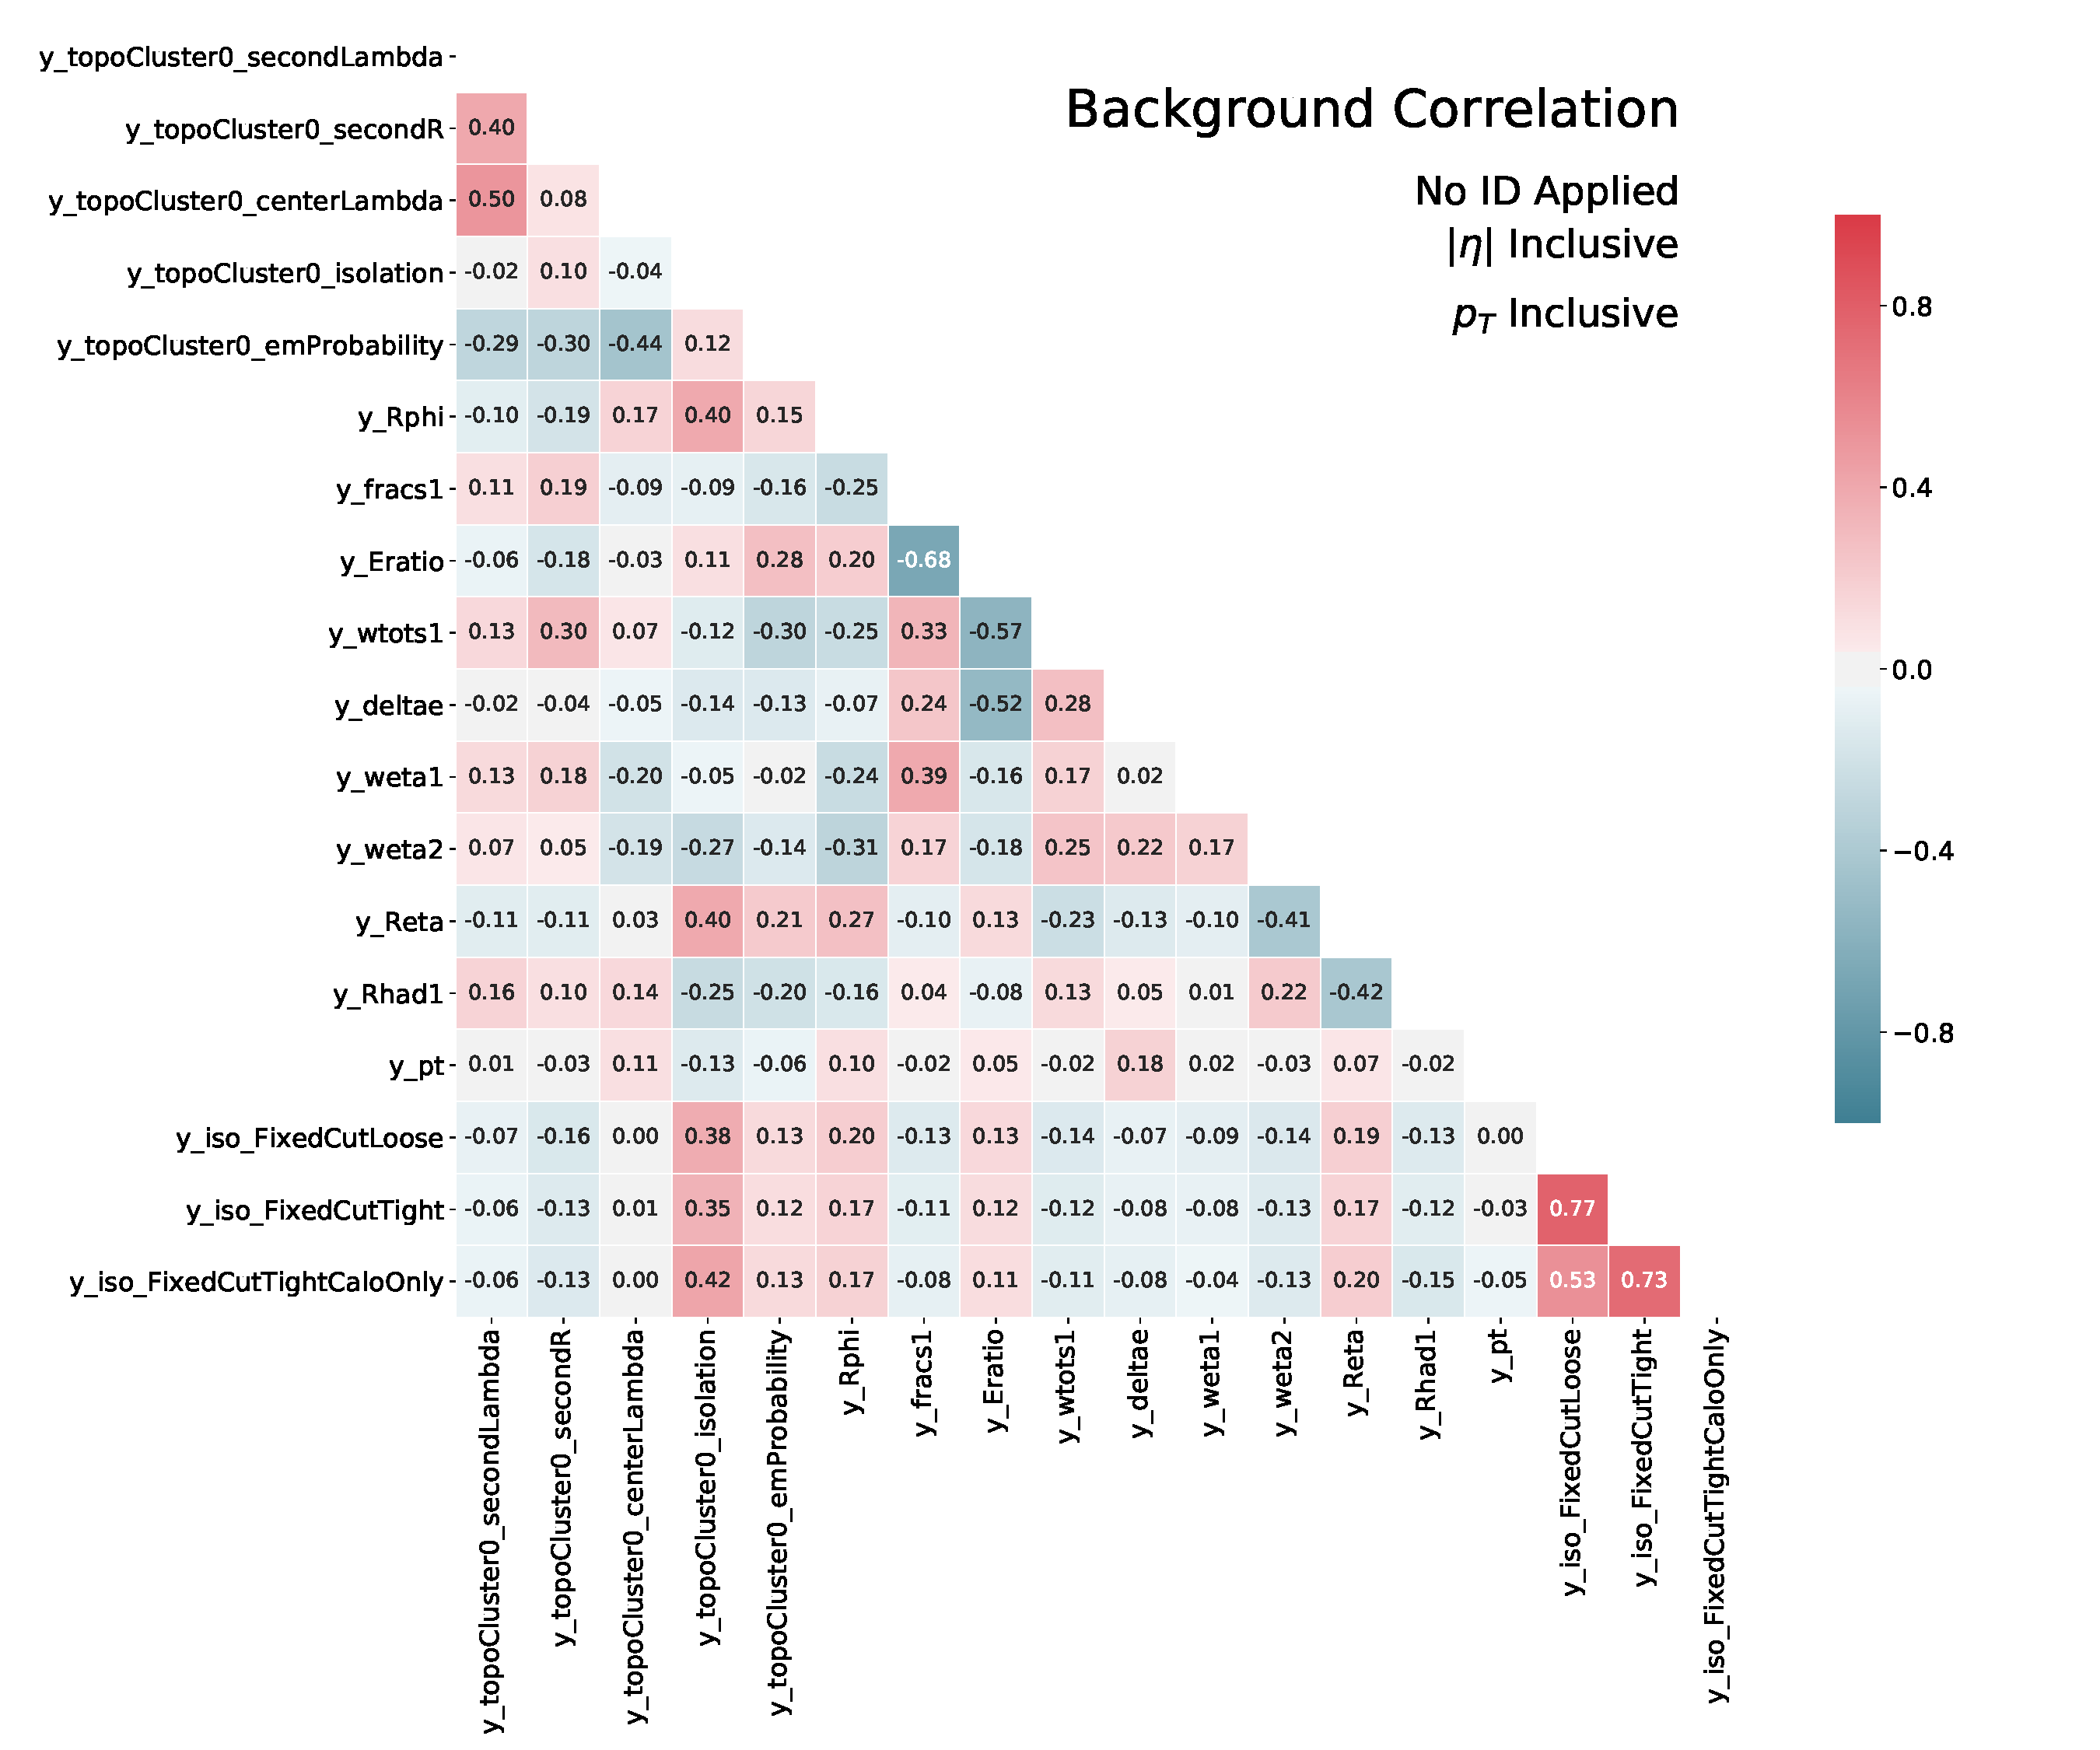
\includegraphics[width=\textwidth]{chapters/chapter4_photonID/images/bkg_none_corr.pdf}
    \caption[Correlation values between the shower shape variables, topological cluster variables, and isolation working points for the jet-fakes sample] {Correlation values between the shower shape variables, topological cluster variables, and isolation working points for the jet-fakes sample.}
    \label{fig:photonid-corrs-bkg}
\end{figure}

\subsection{Incorporating into Photon Identification}

The topological cluster variables were added to the existing shower shape variable-based photon identification. The cut-based approach is reoptimized including the new variables, and new cuts are derived in each \etaPt bin. To compare improvement across bins, the figure of merit used is the improvement in background rejection for the same signal efficiency as the current method, given as

\begin{align}
    Z_{\text{rel}} &= \frac{(1-\epsilon_{bkg,i}) - (1-\epsilon_{bkg,0})}{(1-\epsilon_{bkg,0})} = \frac{\epsilon_{bkg,0} - \epsilon_{bkg,i}}{1-\epsilon_{bkg,0}},
    \label{eqn:improvement-metric}
\end{align}
for relative gain $Z_{\text{rel}}$ (the figure of merit), and background efficiency $\epsilon_{bkg}$ (thus, background rejection is $(1-\epsilon_{bkg}$), where index $i$ indicates the reoptimized photon identification, and index $0$ indicates the shower shape-only identification. This value is calculated bin-wise in \etaPt and shown in Figure~\ref{fig:gain-topo-clusters-added-unconverted}. In principle, adding additional variables to a cut-based method should only improve optimization if the search over possible cut values is exhaustive. However, in several bins, worse performance is found by incorporating new variables. This can be the result of two causes:
\begin{itemize}
    \item In a high dimensional space, such a grid search becomes computationally prohibitive, so a Genetic Algorithm\footnote{The Genetic Algorithm used is a standard method implemented in \texttt{TMVA}, and the details of implementation can be found in Reference~\cite{TMVA}.}~\cite{genetic-algo} is used to find an approximate solution. Increasing dimensionality increases the probability to find local minima that differ from the global minimum, and thus suboptimal solutions.
    \item Statistical fluctuations. Models are trained on an orthogonal subset of events than they are evaluated on, and statistical fluctuations in these samples can influence reported gain, particularly in low stats bins. Figure~\ref{fig:photonid-events} shows the number of signal and background events in each \etaPt bin.
\end{itemize}
%\footnote{These plots, and the remainder of the plots shown in this chapter were created using the \texttt{Seaborn} library~\cite{seaborn} and data manipulation was performed in \texttt{Pandas}~\cite{pandas}.}
\begin{figure}[!hp]
    \centering
    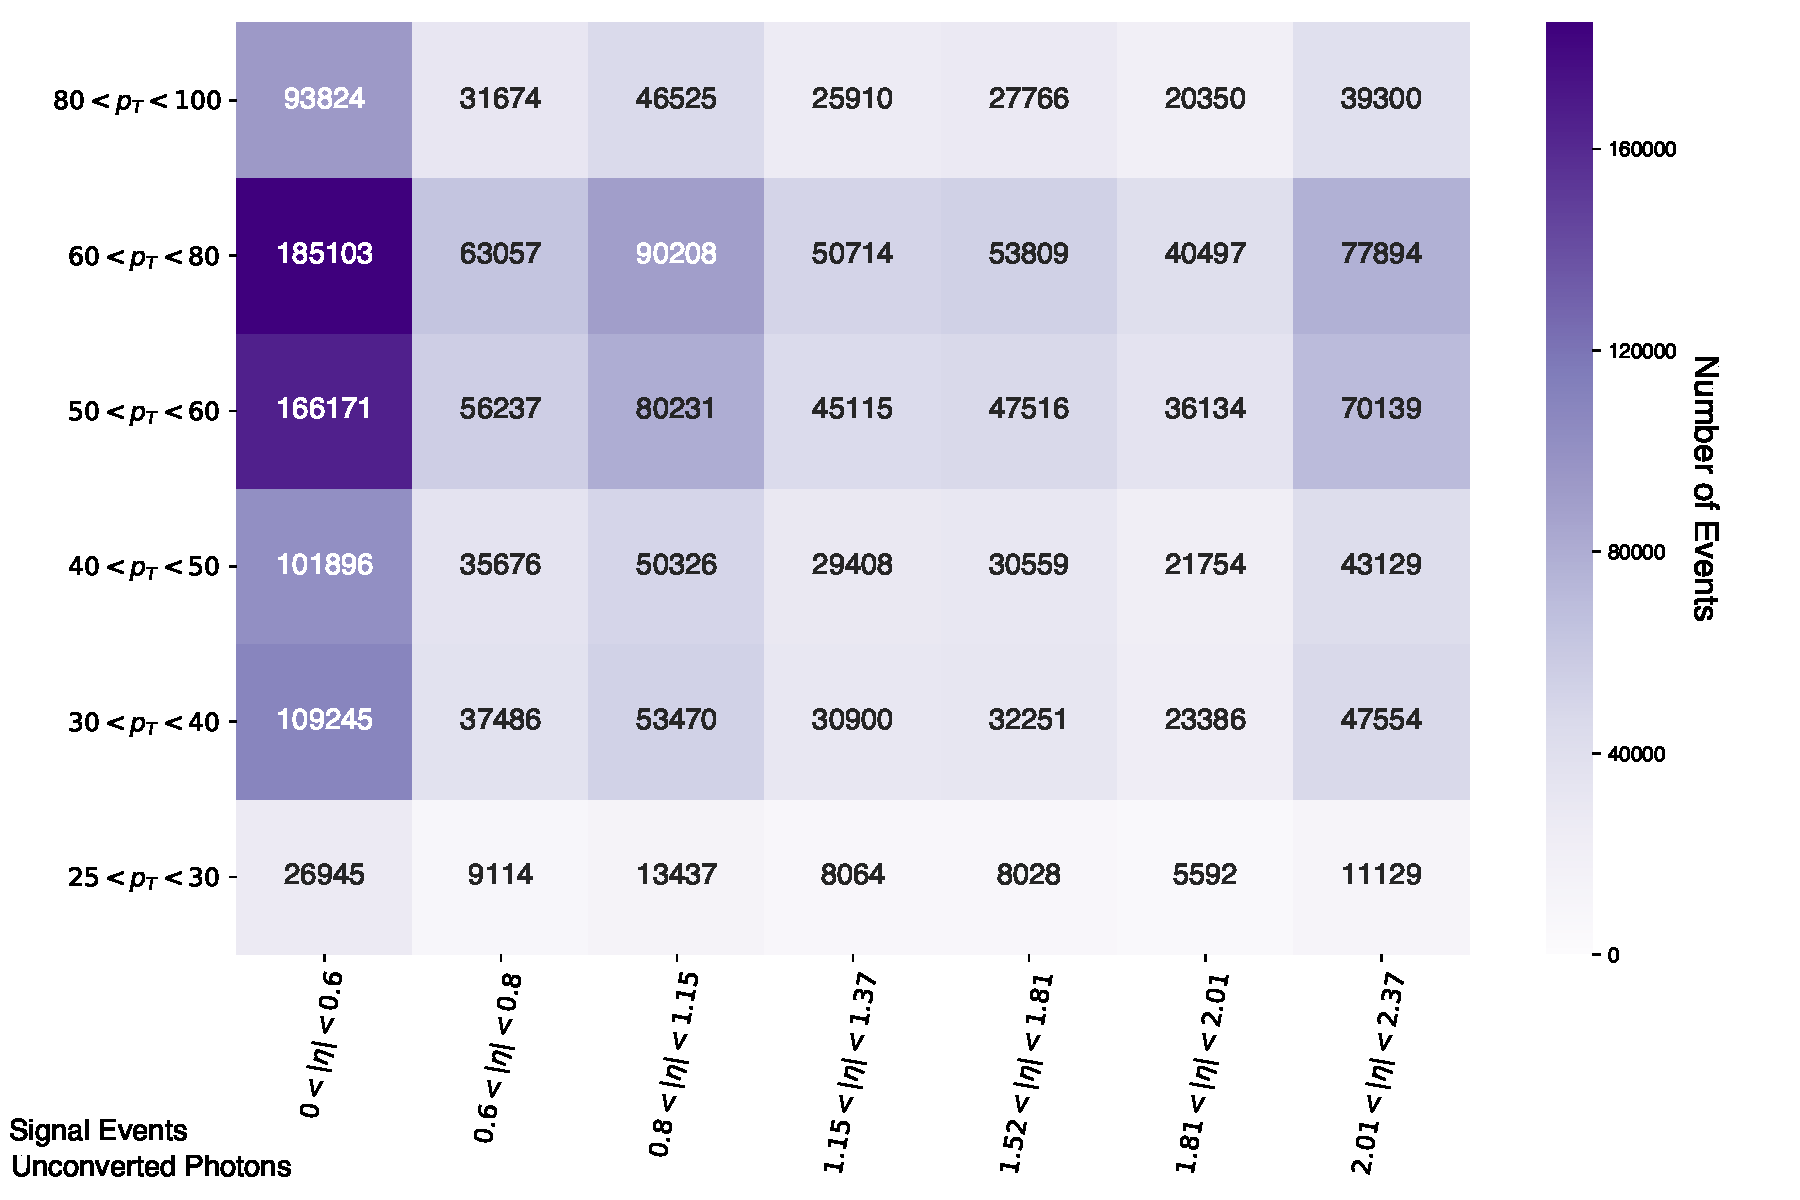
\includegraphics[width=.85\textwidth]{chapters/chapter4_photonID/images/sig_events.pdf}
    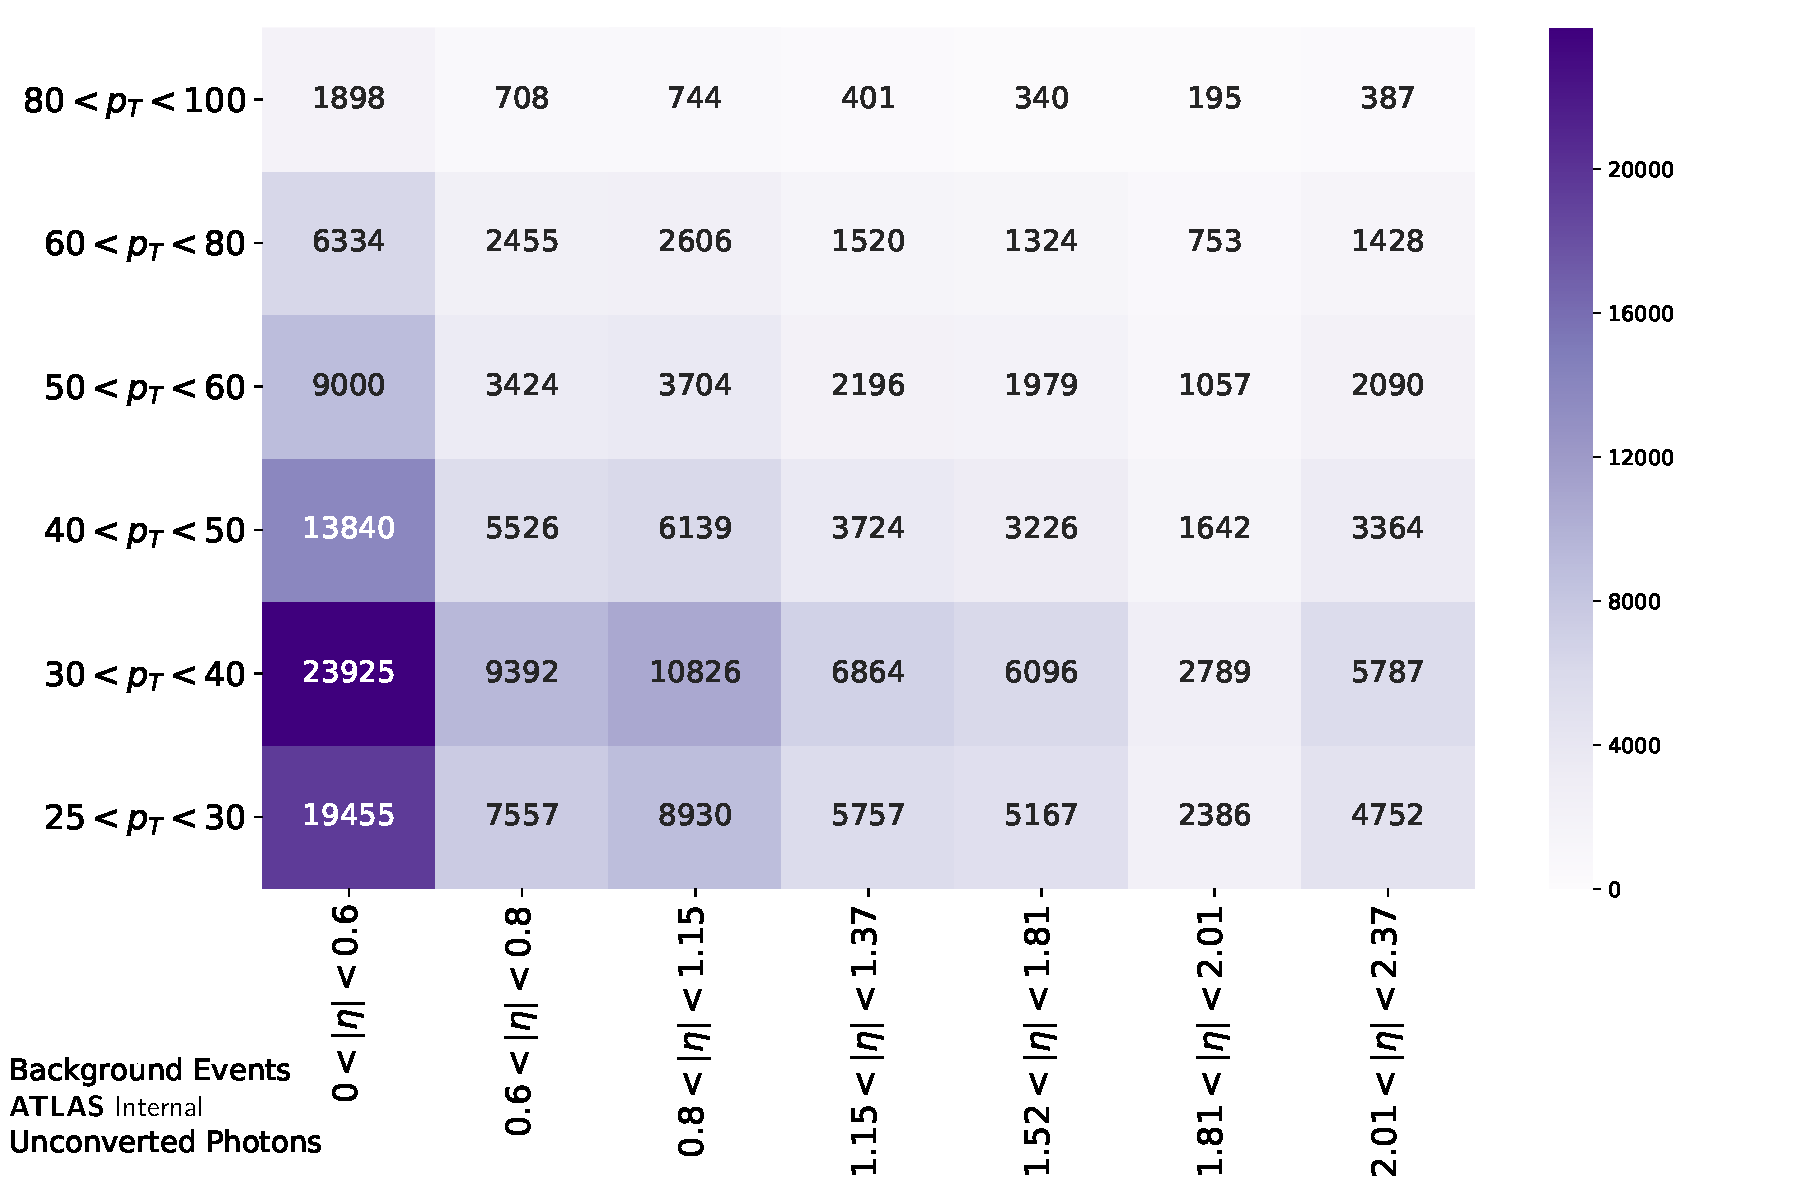
\includegraphics[width=.85\textwidth]{chapters/chapter4_photonID/images/bkg_events.pdf}
    \caption[Number of training events used in the model for unconverted photons in each \etaPt bin for the signal $\gamma$+jets sample, and the background jet fakes sample]{Number of training events used in the model for unconverted photons in each \etaPt bin for the signal $\gamma$+jets sample (top), and the background jet fakes sample (bottom). The preselection described in Section~\ref{sec:photon-id-samples} is used.}
    \label{fig:photonid-events}
\end{figure}

\begin{figure}[!htbp]
    \centering
    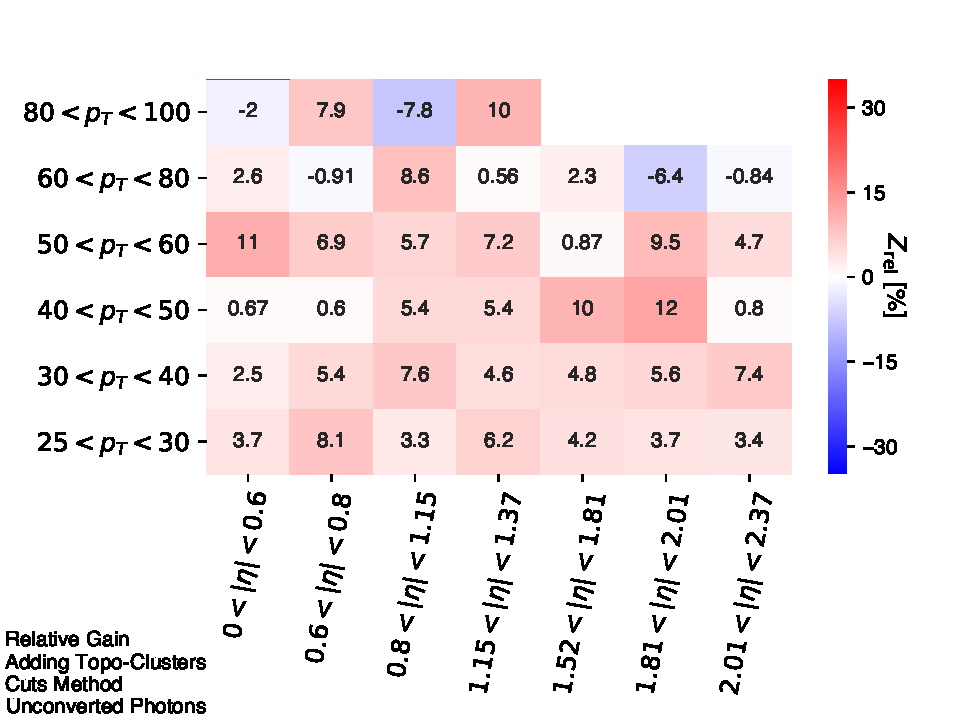
\includegraphics[width=.85\textwidth]{chapters/chapter4_photonID/images/gain_topoAdded_unconverted.pdf}
    \caption[The relative gain in background rejection, $Z_{\text{rel}}$, for each \etaPt bin at 85\% signal efficiency by adding topo-cluster moment variables into the cut-based photon identification menu]{The relative gain in background rejection, $Z_{\text{rel}}$, for each \etaPt bin at 85\% signal efficiency by adding topo-cluster moment variables into the cut-based photon identification menu. Bins with fewer than 400 background events are masked.}
    \label{fig:gain-topo-clusters-added-unconverted}
\end{figure}
As shown in Figure~\ref{fig:gain-topo-clusters-added-unconverted}, by adding these variables as inputs, as much as a 12\% improvement in background rejection for the same signal efficiency can be achieved.
%TODO: add converted?

\section{Multivariate Analysis Techniques}\label{sec:mva-yid}

The current photon identification working points are defined by a univariate rectangular cuts method. Cut optimization is performed through a 9-dimensional scan over the shower shape variables. In order to better reject background, a multivariate approach to defining these working points has been investigated. \gls{MVA} methods are described in detail in Appendix~\ref{app:MVA}, and this section will discuss the improvements brought to photon identification through implementing them. The methods investigated are a \gls{BDT}, described in Section~\ref{ssec:yid-bdt}, and a \gls{NN}, described in Section~\ref{ssec:yid-nn}.


\subsection{Boosted Decision Tree}\label{ssec:yid-bdt}

A gradient boosted \gls{BDT} was employed as an alternative classification algorithm. These models are built using \texttt{TMVA}~\cite{TMVA}. In training, performance suffered heavily from the lack of background training statistics when segmenting into \etaPt bins. To navigate this problem, rather than training an independent model for each \etaPt bin, \pt inclusive models were trained. As shown in Figures~\ref{fig:photonid-corrs-sig} and~\ref{fig:photonid-corrs-bkg}, the input variables have low correlation to \pt, and thus this does not bias the model. This provided better performance in high \pt bins. In low \pt bins, it provided better performance overall, but in a few bins had equivalent or negligibly worse performance. The percent improvement, as defined using the same metric defined in Equation~\ref{eqn:improvement-metric}, is shown in Figure~\ref{fig:bdtinclusive-vs-bdt}, with the bin-wise trained \gls{BDT} used as the baseline.

\begin{figure}[!htbp]
    \centering
    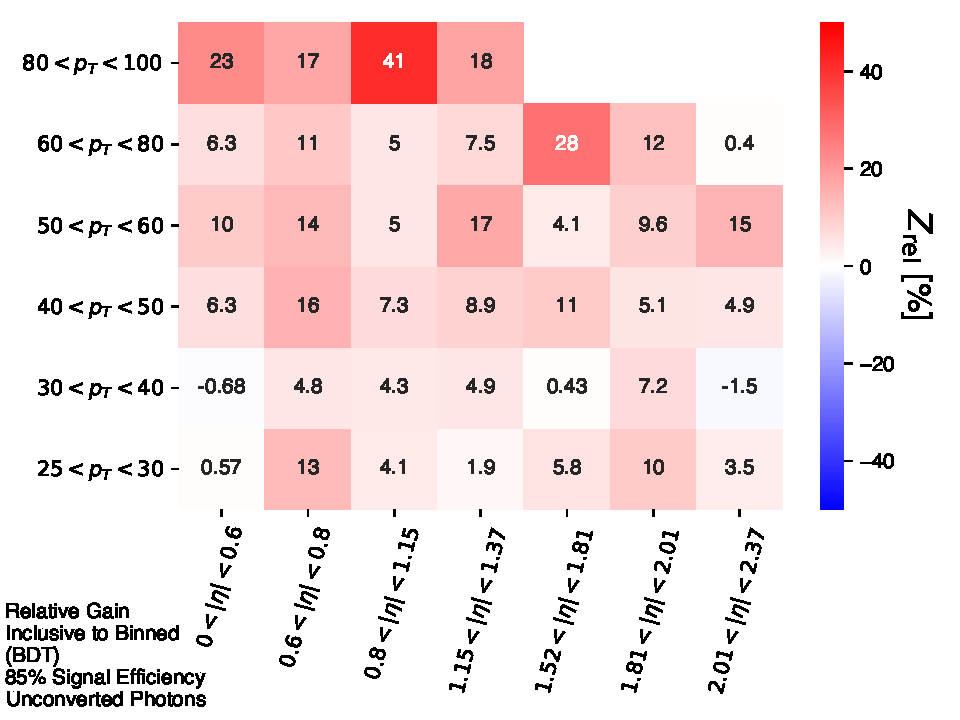
\includegraphics[width=.85\textwidth]{chapters/chapter4_photonID/images/BDTInclusive_v_BDT_normed.pdf}
    \caption[The relative gain in background rejection by using a \pt-inclusive trained \gls{BDT} compared to a \pt-binned \gls{BDT}]
    {The relative gain in background rejection, $Z_{\text{rel}}$, for each \etaPt bin at 85\% signal efficiency by using a \pt-inclusive trained \gls{BDT} compared to a \pt-binned \gls{BDT}. Only shower-shape variables are included as inputs. Bins with fewer than 400 background events are masked.}
    \label{fig:bdtinclusive-vs-bdt}
\end{figure}


To see the improvement over the cut-based method, the \gls{BDT} is compared to the current photon identification, using the same figure of merit (Equation~\ref{eqn:improvement-metric}), where the efficiency denoted $i$ now represents the \gls{BDT} model, and the efficiency denoted $0$ represents the current cut-based model. This model performs better in the majority of bins, by as much as 22\%, but performs worse in all of the outer \abseta bins where there are poor background statistics, shown in Figure~\ref{fig:gain-bdt-vs-cuts}.
\begin{figure}[!htbp]
    \centering
    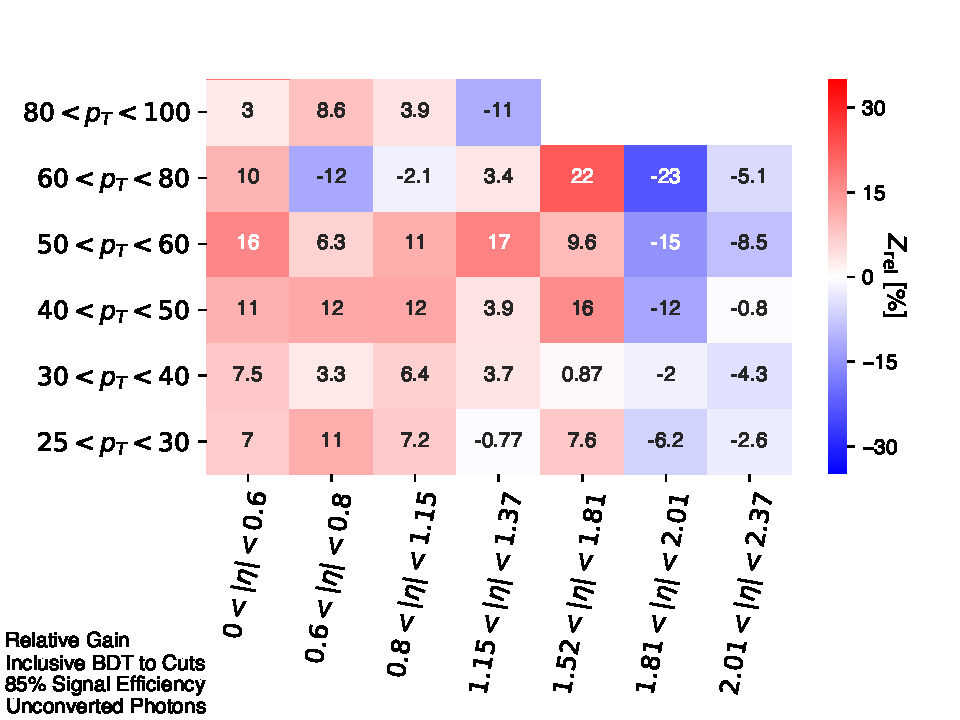
\includegraphics[width=.85\textwidth]{chapters/chapter4_photonID/images/gain_BDTinclusive_cuts_unconverted.pdf}
    \caption[The relative gain in background rejection by using a \gls{BDT} compared to the cut-based photon identification menu]
    {The relative gain in background rejection, $Z_{\text{rel}}$, for each \etaPt bin at 85\% signal efficiency by using a \gls{BDT} compared to the cut-based photon identification menu. Only shower-shape variables are included as inputs. Bins with fewer than 400 background events are masked.}
    \label{fig:gain-bdt-vs-cuts}
\end{figure}


\subsection{Neural Network}\label{ssec:yid-nn}

In addition to a \gls{BDT}, a \gls{NN} was studied for photon classification, considering the same shower shape variables. The model topology\footnote{A description of \gls{NN} topologies, activation functions, and other associated terminology can be found in Appendix~\ref{app:MVA}.} used is shown in Figure~\ref{fig:nn-model}, it has an input layer of size 9 to match the number of shower shape variables, which is densely connected to a hidden layer of size 6, with ReLU activation functions. This layer is densely connected to an output with a sigmoid activation function. A dropout~\cite{dropout} of 20\% is used on the hidden layer while training to reduce overtraining. This produces a total of 67 trainable parameters. Models with additional layers and with a wider hidden layer were investigated but found to not provide any additional improvement in background rejection, so were rejected.

% It was developed using Keras~\cite{Keras} with the Tensorflow~\cite{Tensorflow} backend.
%\footnote{Data manipulation was performed using the \texttt{Numpy}~\cite{numpy} library.}

\begin{figure}[!htbp]
    \centering
    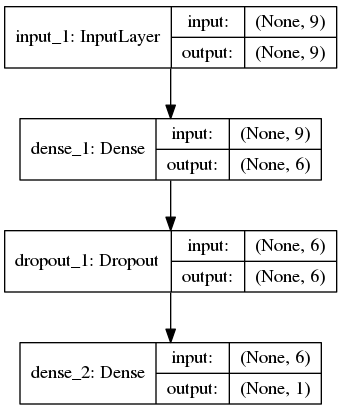
\includegraphics[width=.30\textwidth]{chapters/chapter4_photonID/images/model.png}
    \caption[A diagram of the \gls{NN} topology used for photon identification]
    {A diagram of the \gls{NN} topology used for photon identification. Inputs to this \gls{NN} are the shower shape variables.}
    \label{fig:nn-model}
\end{figure}

The \gls{NN} performed better at low \pt than the inclusively trained \gls{BDT} by as much as 30\%, but worse at high \pt. This comparison can be seen in Figure~\ref{fig:nn-v-bdt-unconverted}. A \pt-inclusive training approach was considered for the \gls{NN} as well, however provided a worse performance for the majority of \etaPt bins, shown in Figure~\ref{fig:nninclusive-v-binned}.

\begin{figure}[!htbp]
    \centering
    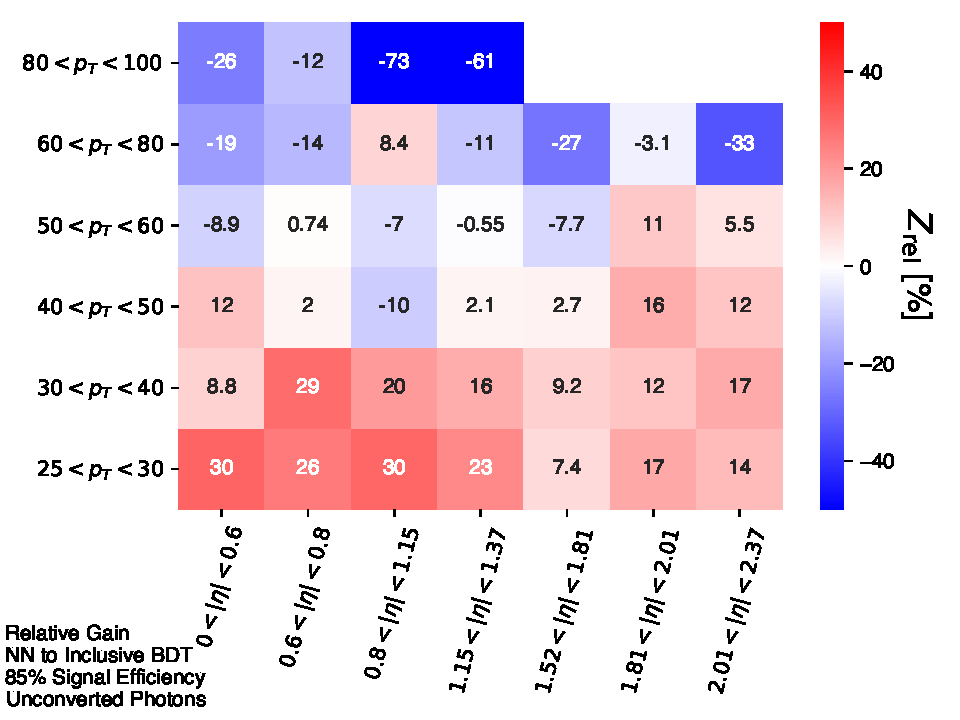
\includegraphics[width=.85\textwidth]{chapters/chapter4_photonID/images/NN_v_BDTinclusive_normed.pdf}
    \caption[The relative gain in background rejection by using a \gls{NN} trained bin-wise compared to a \gls{BDT} trained inclusively]
    {The relative gain in background rejection, $Z_{\text{rel}}$, for each \etaPt bin at 85\% signal efficiency by using a \gls{NN} trained in each \etaPt bin compared to a \gls{BDT} trained inclusively. Negative values can be interpreted as the \gls{BDT} having better performance than the \gls{NN}. Only shower-shape variables are included as inputs for both models. Bins with fewer than 400 background events are masked.}
    \label{fig:nn-v-bdt-unconverted}
\end{figure}


\begin{figure}[!htbp]
    \centering
    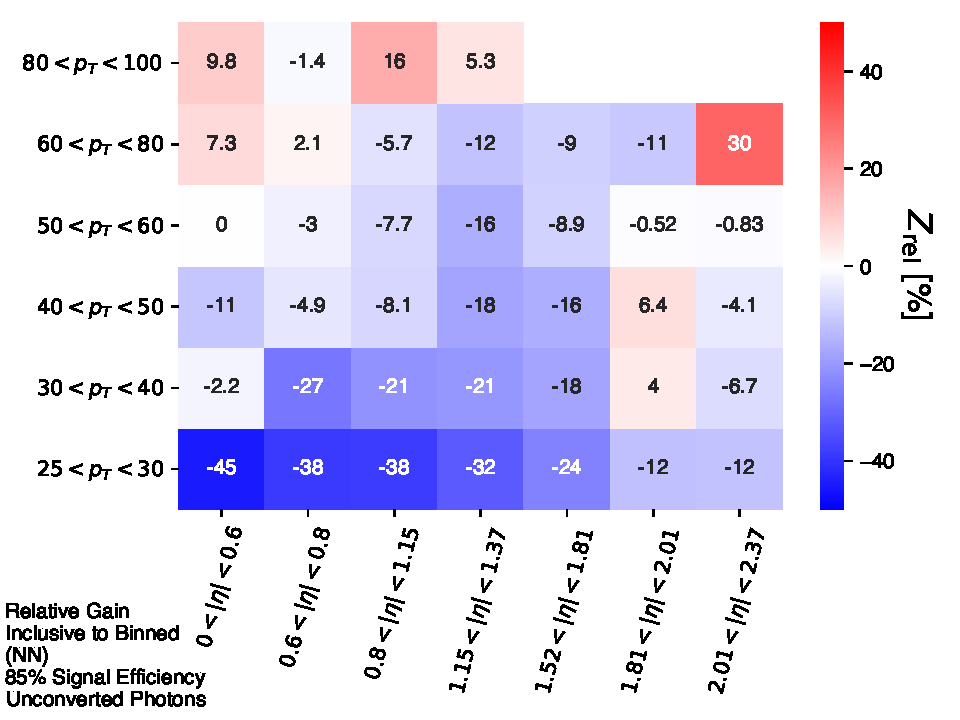
\includegraphics[width=.85\textwidth]{chapters/chapter4_photonID/images/NNinclusive_v_NN_normed.pdf}
    \caption[The relative gain in background rejection by using a \gls{NN} trained inclusively compared to one trained bin-wise]
    {The relative gain in background rejection, $Z_{\text{rel}}$, for each \etaPt bin at 85\% signal efficiency by using a \gls{NN} trained inclusively compared to one trained in each \etaPt bin. Negative values can be interpreted as the bin-wise training having better performance than the inclusive training. Only shower-shape variables are included as inputs for both models. Bins with fewer than 400 background events are masked.}
    \label{fig:nninclusive-v-binned}
\end{figure}



\subsection{MVA With Topo-Cluster Variables}

The \gls{BDT} was studied incorporating the topo-cluster moments as inputs. The relative gain when doing so is shown in Figure~\ref{fig:bdt-topo-vs-cuts}, as compared to the current tight photon identification working point using the cut-based method. Through applying this optimization, as much as a 27\% improvement is shown, and in most \etaPt bins, a gain of greater than 10\% is shown.
\begin{figure}[!htbp]
    \centering
    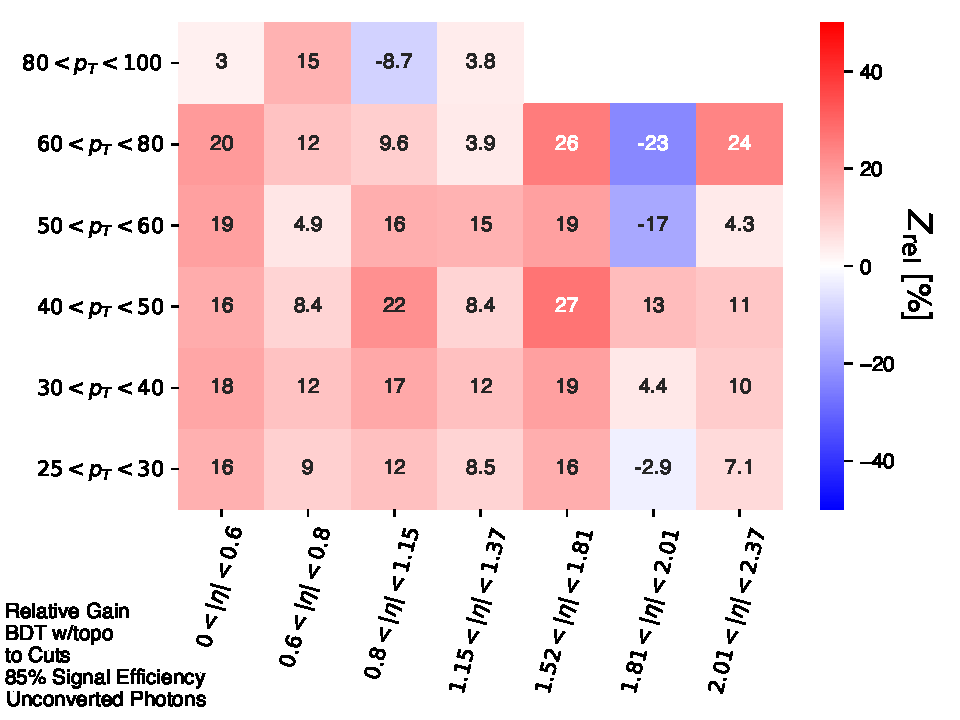
\includegraphics[width=.85\textwidth]{chapters/chapter4_photonID/images/BDTtopo_v_cuts_normed.pdf}
    \caption[The relative gain in background rejection by using a \gls{BDT} with topo-cluster variables compared to the current tight photon identification methods]
    {The relative gain in background rejection, $Z_{\text{rel}}$, for each \etaPt bin at 85\% signal efficiency by using a \gls{BDT} with the topo-cluster variables as input in addition to the shower shape variables compared to the current tight photon identification cut-based method. Bins with fewer than 400 background events are masked.}
    \label{fig:bdt-topo-vs-cuts}
\end{figure}

\section{Conclusion}

Through adding topo-cluster moments as inputs and by switching to a \gls{BDT}, an improvement of greater than 10\% in background rejection for the same signal efficiency as the tight working point is demonstrated in most \etaPt bins, and as much as a 27\% improvement is shown. While the comparison between data and \gls{MC} modeling for the topo-cluster moments already demonstrates reasonably good agreement, proper calibration must be performed before full implementation. 

The presented analysis in this thesis, studying \hhyybb production, has two photons in the final state. These per-photon improvements can lead to a improvement, since the signal selection is sensitive to the square of the photon identification efficiency. The analysis is statistics limited, the signal significance effectively scales as the number of signal events, so the ability to loosen the signal selection will directly improve the final analysis sensitivity.